% % % % % % % % %  MDT UFSM 2021  % % % % % % % % %
%% Arquivo base para o documento - ver. 1.0 %%
% % % % % % % % % % % % % % % % % % % % % % % % %

\documentclass[oneside,openright,12pt]{ufsm_2021}
\usepackage{listings}
\usepackage[scaled]{helvet}
\renewcommand*\familydefault{\sfdefault}
\usepackage{lipsum}
\usepackage{quoting}
\usepackage{tikz}
\usetikzlibrary{positioning,shapes.geometric}
\usepackage{xcolor}
% Pendências visíveis no PDF; remover antes da entrega.
\newcommand{\verificar}[1]{\textcolor{red}{[VERIFICAR: #1]}}
% Só valem se a classe não definir estes comandos (abntex2cite define \citeonline).
\providecommand{\citeonline}{\cite}
\providecommand{\fonte}[1]{\par\vspace{2pt}{\small Fonte: #1}}
\usepackage{array}
\newcolumntype{L}[1]{>{\raggedright\arraybackslash}p{#1}}

% % % DADOS DO TRABALHO % % %

% % INSTITUCIONAIS
\centroensino{COLÉGIO POLITÉCNICO}
\centroensinosigla{CCNE}
\nivelensino{Graduação}
\curso{Sistemas para Internet}
\ppg{PPGALGO}
\statuscurso{Curso}
\cidade{Santa Maria}
\estado{RS}

% % AUTOR
\author{João Víctor Guedes}
\sexo{M}
\grauensino{Graduação}
\grauobtido{Tecnólogo}
\email{joaoguedes1404@gmail.com}

% % BANCA
\orientador{Alencar Machado}{Dr}{UFSM}{M}{P}
\bancaum{Vinicius Maran}{Dr}{UFSM}{F}{M}
\bancadois{Pedro Bilar}{Pg}{UFSM}

% % TÍTULO
% Título provisório, adaptado do artigo ICEIS.
\titulo{RAG EM PLATAFORMAS GOVERNAMENTAIS:}
\englishtitle{RAG in Government Platforms:}
\subtitulo{PARECERES TÉCNICOS ASSISTIDOS POR LLM NA CERTIFICAÇÃO HIGIÊNICO-SANITÁRIA DA PNIP.}
\subenglishtitle{LLM-Assisted Technical Opinions for Hygiene-Sanitary Certification in PNIP.}
\areaconcentracao{Inteligência Artificial e Computação Aplicada.}

\tccg
\data{30}{06}{2026}

% % EPIGRAFE
\epigrafe{"Uma lição sem dor não tem sentido. Porque as pessoas não podem ganhar algo sem sacrificar algo em troca."}{Edward Elric}
% % DEDICATORIA
\dedicatoria{
	Dedico esse trabalho a minha família por todo o suporte dado durante a minha jornada acadêmica, mas principalmente
	a minha mãe Joceli Maria de Mattos e ao meu pai Rubens Rodrigo Schultz Guedes, que sempre fizeram de tudo para que eu consiga apenas focar na parte acadêmica sem 
	ter que me preocupar com mais nada. Agradeço também a minha namorada Ana Caroline Souza Santos, que sempre me apoiou e incentivou durante toda a minha trajetória, mesmo nos momentos mais difíceis.
}
% % AGRADECIMENTOS
\agradecimentos{
	Agradeço ao meu orientador, Prof. Dr. Alencar Machado, pela orientação, paciência e contribuição para a realização deste trabalho.
	Agradeço também ao Laboratório de Computação Ubíqua Móvel e Aplicada (LUMAC) pela oportunidade de aplicar os meus conhecimentos adquiridos dentro do curso na prática.
	Agradeço também aos professores do curso de Sistemas para Internet pelos conhecimentos compartilhados e pela paciência durante a passagem do mesmo.
	Por fim, agradeço a minha família e amigos pelo apoio, incentivo e conselhos durante toda essa jornada. 
}

% % RESUMO
% Escrever ao final. O resumo do artigo ICEIS (artigo-iceis-guedes/pt-br/main.tex) serve de base.
\resumo{
\verificar{resumo a escrever quando os capítulos de resultados estiverem prontos.}
}
\palavrachave{\textit{Retrieval-Augmented Generation. Large Language Models. Governo Digital. PNIP. Certificação Higiênico-Sanitária.}}

% % ABSTRACT
\abstract{
\verificar{abstract to be written.}
}
\keywords{\textit{Retrieval-Augmented Generation. Large Language Models. Digital Government. PNIP. Hygiene-Sanitary Certification.}}

% % LISTAS
\abreviaturamax{SIGLAMAX}
\listadeabreviaturas{
	BGE-M3 & \textit{BAAI General Embedding M3} \\
	DPR & \textit{Dense Passage Retrieval} \\
	HNSW & \textit{Hierarchical Navigable Small World} \\
	HS & Higiênico-Sanitária \\
	IA & Inteligência Artificial \\
	JAP & Junta Administrativa de Recursos de Infrações \\
	LGPD & Lei Geral de Proteção de Dados Pessoais \\
	LLM & \textit{Large Language Model} \\
	LoRA & \textit{Low-Rank Adaptation} \\
	LUMAC & Laboratório de Computação Ubíqua, Móvel e Aplicada \\
	MAPA & Ministério da Agricultura e Pecuária \\
	MPA & Ministério da Pesca e Aquicultura \\
	OCR & \textit{Optical Character Recognition} \\
	PAC & Programa de Autocontrole \\
	PDSA-RS & Plataforma de Defesa Sanitária Animal do Rio Grande do Sul \\
	PNIP & Plataforma Nacional da Indústria do Pescado \\
	RAG & \textit{Retrieval-Augmented Generation} \\
	RLHF & \textit{Reinforcement Learning from Human Feedback} \\
	SEAPI-RS & Secretaria da Agricultura, Pecuária e Desenvolvimento Rural do Rio Grande do Sul \\
	UFSM & Universidade Federal de Santa Maria
}

\siglamax{SIGLAMAX}
\listadesiglas{
	BGE-M3 & \textit{BAAI General Embedding M3} \\
	DPR & \textit{Dense Passage Retrieval} \\
	HNSW & \textit{Hierarchical Navigable Small World} \\
	HS & Higiênico-Sanitária \\
	IA & Inteligência Artificial \\
	JAP & Junta Administrativa de Recursos de Infrações \\
	LGPD & Lei Geral de Proteção de Dados Pessoais \\
	LLM & \textit{Large Language Model} \\
	LoRA & \textit{Low-Rank Adaptation} \\
	LUMAC & Laboratório de Computação Ubíqua, Móvel e Aplicada \\
	MAPA & Ministério da Agricultura e Pecuária \\
	MPA & Ministério da Pesca e Aquicultura \\
	OCR & \textit{Optical Character Recognition} \\
	PAC & Programa de Autocontrole \\
	PDSA-RS & Plataforma de Defesa Sanitária Animal do Rio Grande do Sul \\
	PNIP & Plataforma Nacional da Indústria do Pescado \\
	RAG & \textit{Retrieval-Augmented Generation} \\
	RLHF & \textit{Reinforcement Learning from Human Feedback} \\
	SEAPI-RS & Secretaria da Agricultura, Pecuária e Desenvolvimento Rural do Rio Grande do Sul \\
	UFSM & Universidade Federal de Santa Maria
}

% % FICHA CATALOGRAFICA
\semcatalografica

\videoconferenciabancap{}
\videoconferenciabancas{}
\providecommand{\deactivatetocstyle}{}
\providecommand{\reactivatetocstyle}{}

\begin{document}

\pretextual

% % CAPÍTULOS
% ============================================================
% Capítulo 1 - Introdução
% Base: artigo ICEIS (artigo-iceis-guedes/pt-br/main.tex), Seção 1.
% ============================================================
\chapter{Introdução}
\label{cap:introducao}

Os \textit{Large Language Models} (LLMs) passaram, em poucos anos, de objeto de pesquisa a ferramenta de uso cotidiano. Treinados sobre grandes volumes de texto, esses modelos geram, resumem e respondem perguntas com pouca ou nenhuma supervisão específica para cada tarefa \cite{Brown2020,Zhao2023}. Essa capacidade chamou a atenção da administração pública, em que os órgãos lidam com muitos documentos e precisam interpretar normas extensas, técnicas e que mudam com o tempo. A literatura recente registra aplicações de LLMs na gestão de documentos oficiais \cite{Ayuyang2026}, na verificação de conformidade regulatória \cite{Legado2026}, em processos de compras públicas \cite{Sofat2024} e no apoio a decisões administrativas \cite{Drobotowicz2026,Montero2026}, além de iniciativas para regular o uso dessas ferramentas no próprio governo brasileiro \cite{Alves2024}.

Em sistemas governamentais, porém, uma resposta útil não basta: ela precisa ser correta, rastreável até a norma que a fundamenta e verificável por quem responde pela decisão. Os LLMs não oferecem essas garantias por si mesmos. Seu conhecimento fica limitado ao que estava nos dados de treinamento, e eles podem produzir afirmações plausíveis, mas falsas, fenômeno conhecido como alucinação \cite{Ji2023}. A \textit{Retrieval-Augmented Generation} (RAG) \cite{Lewis2020} trata dessas limitações ao acrescentar ao \textit{prompt} trechos recuperados de uma base de conhecimento externa, de modo que a resposta se apoie em documentos autorizados e possa citá-los \cite{Gao2023}. Como a base pode ser atualizada sem retreinar o modelo, a abordagem é adequada a domínios regulados, em que as normas são publicadas, alteradas e revogadas com frequência.

No Laboratório de Computação Ubíqua, Móvel e Aplicada (LUMAC) da Universidade Federal de Santa Maria (UFSM), essa linha de pesquisa começou na Plataforma de Defesa Sanitária Animal do Rio Grande do Sul (PDSA-RS). Ali, um sistema RAG que recupera trechos das instruções normativas sobre sanidade avícola elevou de 12\% para 55\% a acurácia das respostas de um LLM executado localmente na análise de solicitações de certificação \cite{Montero2025iceis,Montero2025}. Em seguida, o grupo propôs uma arquitetura de assistente para analistas do setor público e avaliou pareceres gerados por LLM em recursos administrativos julgados pela Junta Administrativa de Processos (JAP) da Secretaria da Agricultura, Pecuária, Produção Sustentável e Irrigação do Rio Grande do Sul (SEAPI-RS) \cite{Montero2026}. Essa arquitetura foi depois implementada como a plataforma DocFlow, usada neste trabalho.

Este trabalho leva essa abordagem a um novo contexto: a Plataforma Nacional da Indústria do Pescado (PNIP) \cite{MPA2024}, a plataforma digital oficial do Ministério da Pesca e Aquicultura (MPA) para a certificação de embarcações e produtos pesqueiros. Entre os processos tratados na PNIP está a certificação higiênico-sanitária (HS) de embarcações, regida pela Portaria SAP/MAPA nº~310/2020 e suas alterações \cite{Portaria310,Portaria171,Portaria742}. Em cada solicitação, o técnico responsável pela embarcação anexa documentos e registros fotográficos que comprovam os requisitos da norma, e um analista do MPA confere cada item da lista de verificação, registra as não conformidades e redige um parecer técnico.

\section{Problema}
\label{sec:problema}

O gargalo da certificação HS é a carga de trabalho. Há mais solicitações do que os analistas disponíveis conseguem examinar, e muitas ficam paradas na plataforma aguardando análise. Cada análise exige ler um dossiê heterogêneo, com programas de autocontrole, laudos, declarações, registros de treinamento e dezenas de fotografias, e confrontá-lo com uma norma que já foi alterada mais de uma vez. Um LLM poderia ler o dossiê e as fotos, confrontá-los com as normas aplicáveis e redigir um rascunho de parecer para o analista revisar, mantendo com ele a decisão final. Não se sabe, porém, se as técnicas que funcionaram na PDSA-RS, em que a decisão depende de dados estruturados de exames laboratoriais, se transferem para um processo em que a decisão depende do julgamento sobre o conteúdo de documentos e fotografias.

Daí a questão que orienta este trabalho: \textbf{a recuperação das normas aplicáveis por RAG e o envio dos registros fotográficos ao modelo ajudam um LLM a reproduzir a análise dos analistas da PNIP na certificação higiênico-sanitária de embarcações?}

\section{Objetivos}
\label{sec:objetivos}

\subsection{Objetivo geral}

Avaliar a aplicação de uma arquitetura RAG com LLMs ao apoio à análise das solicitações de certificação higiênico-sanitária de embarcações na PNIP, medindo se o contexto normativo recuperado e os registros fotográficos aproximam as sugestões do modelo da análise dos analistas humanos.

\subsection{Objetivos específicos}

\begin{enumerate}
	\item Analisar os trabalhos anteriores do grupo na PDSA-RS e situar este trabalho na literatura sobre LLMs e RAG na administração pública, por meio de uma revisão sistemática rápida.
	\item Indexar o corpus normativo da certificação HS segmentado por artigo, preservando a origem de cada trecho para que possa ser citado.
	\item Estender a plataforma DocFlow para recuperar as normas a partir dos documentos de cada processo e para enviar os registros fotográficos aos modelos como imagens.
	\item Avaliar, em processos já decididos, modelos de pesos abertos executados em infraestrutura própria e modelos hospedados, com e sem o contexto normativo e as fotografias, tomando a decisão do analista como referência.
	\item Medir a qualidade da recuperação e comparar, item a item, rascunhos de parecer gerados pelo modelo com os pareceres finais dos analistas.
\end{enumerate}

\section{Justificativa}
\label{sec:justificativa}

A certificação HS atesta as boas práticas higiênico-sanitárias a bordo das embarcações pesqueiras e, junto com as demais certificações da PNIP, sustenta a rastreabilidade que liga cada produto pesqueiro à sua origem \cite{Olsen2018}, um dos instrumentos de combate à pesca ilegal, não declarada e não regulamentada \cite{Agnew2009}. A demora na análise atrasa a regularização das embarcações e sobrecarrega os analistas. Um assistente que adiante a leitura do dossiê e aponte as evidências relevantes pode reduzir esse tempo, desde que suas sugestões sejam rastreáveis e a decisão permaneça com o servidor.

Do ponto de vista científico, a revisão da literatura feita neste trabalho (Capítulo~\ref{cap:trabalhos-relacionados}) não encontrou estudos que gerem pareceres técnicos sobre solicitações de certificação combinando os documentos de um dossiê, seus registros fotográficos e a recuperação das normas aplicáveis. Avaliar essa combinação em processos reais, e relatar também o que não funcionou, contribui para entender os limites do RAG em tarefas de julgamento administrativo. Por fim, a execução local dos modelos de pesos abertos permite processar documentos de terceiros sem enviá-los a serviços externos, o que importa sob a Lei Geral de Proteção de Dados Pessoais \cite{Brasil2018}.

\section{Organização do trabalho}
\label{sec:organizacao}

O Capítulo~\ref{cap:referencial} apresenta os conceitos de inteligência artificial, LLMs, \textit{embeddings}, RAG, \textit{fine-tuning} e \textit{chunking}, a PDSA-RS e o contexto da PNIP e da certificação higiênico-sanitária.
O Capítulo~\ref{cap:trabalhos-relacionados} analisa os trabalhos anteriores do grupo e resume uma revisão sistemática rápida sobre LLMs e RAG na administração pública.
O Capítulo~\ref{cap:metodologia} descreve a plataforma DocFlow e as extensões feitas para a PNIP, o Capítulo~\ref{cap:estudo-caso} relata o estudo de caso, com seu desenho, resultados e discussão, e o Capítulo~\ref{cap:consideracoes} apresenta as dificuldades encontradas, as limitações, os trabalhos futuros e a conclusão.

% ============================================================
% Capítulo 2 - Referencial Teórico
% Bases: artigo ICEIS (pt-br/main.tex), Montero et al. (2025, ICEIS e Information)
% e Montero et al. (2026). Marcadores [VERIFICAR] indicam dados a confirmar.
% ============================================================
\chapter{Referencial Teórico}
\label{cap:referencial}

Este capítulo apresenta os conceitos em que o trabalho se apoia. A Seção~\ref{sec:ia} situa a inteligência artificial e sua evolução; a Seção~\ref{sec:llm} descreve os LLMs; a Seção~\ref{sec:embedding} apresenta os \textit{embeddings}, a representação vetorial de textos em que a recuperação se apoia; a Seção~\ref{sec:chunking}, a divisão dos documentos em trechos, o \textit{chunking}; e a Seção~\ref{sec:rag}, a arquitetura RAG, que combina esses componentes com um LLM. As duas últimas seções descrevem o contexto de aplicação: a PDSA-RS, com os trabalhos anteriores do grupo, e a PNIP, com a certificação higiênico-sanitária de embarcações.

% ------------------------------------------------------------
\section{Inteligência Artificial}
\label{sec:ia}

A inteligência artificial (IA) é o campo da computação que estuda e constrói sistemas capazes de executar tarefas que, quando feitas por pessoas, exigem inteligência, como raciocinar, reconhecer padrões, compreender a linguagem e tomar decisões \cite{Russell2020}. A pergunta sobre se máquinas podem pensar foi formulada por \citeonline{Turing1950}, que propôs substituí-la por um teste operacional, o jogo da imitação. O termo ``inteligência artificial'' surgiu poucos anos depois, na proposta do seminário de Dartmouth de 1956, que partia da conjectura de que todo aspecto da aprendizagem ou da inteligência poderia ser descrito com precisão suficiente para ser simulado por uma máquina \cite{McCarthy2006}.

\subsection{Da IA simbólica ao aprendizado de máquina}

As primeiras décadas foram dominadas pela IA simbólica, em que o conhecimento é representado explicitamente por regras e símbolos manipulados por algoritmos de busca e inferência lógica. Os sistemas especialistas, que codificavam em regras o conhecimento de especialistas humanos, tiveram aplicação comercial nas décadas de 1970 e 1980, mas mostraram-se caros de construir e manter e frágeis diante de situações não previstas pelas regras \cite{Russell2020}. Essas dificuldades, somadas a expectativas não cumpridas, levaram a períodos de redução de investimento conhecidos como ``invernos da IA''.

O aprendizado de máquina mudou a abordagem: em vez de escrever as regras, o sistema as induz a partir de exemplos \cite{Bishop2006}. No aprendizado supervisionado, o modelo aprende a mapear entradas em saídas a partir de exemplos rotulados; no não supervisionado, procura estrutura em dados sem rótulos; e no aprendizado por reforço, aprende uma política de ações a partir das recompensas que recebe do ambiente \cite{Russell2020}. Em todos os casos, o desempenho passa a depender da quantidade e da qualidade dos dados, e não apenas do conhecimento que o projetista consegue explicitar.

\subsection{Redes neurais e aprendizado profundo}

As redes neurais artificiais são modelos compostos por camadas de unidades que calculam somas ponderadas de suas entradas seguidas de funções de ativação não lineares. O algoritmo de retropropagação do erro \cite{Rumelhart1986} tornou viável treinar redes com camadas intermediárias, ajustando os pesos por gradiente descendente para minimizar uma função de perda. O aprendizado profundo empilha muitas dessas camadas, de modo que cada uma aprende representações progressivamente mais abstratas dos dados, sem que as características precisem ser definidas manualmente \cite{LeCun2015,Goodfellow2016}.

O marco da retomada foi a vitória de uma rede convolucional profunda na competição ImageNet de 2012 \cite{Krizhevsky2012}, possibilitada por grandes conjuntos de dados rotulados e pelo processamento paralelo em GPUs. Para dados sequenciais, como texto, as redes recorrentes, em particular as LSTM \cite{Hochreiter1997}, foram por anos a arquitetura dominante, até a chegada do Transformer \cite{Vaswani2017}, base dos modelos de linguagem descritos a seguir.

% ------------------------------------------------------------
\section{Large Language Models}
\label{sec:llm}

Um modelo de linguagem é um modelo computacional que atribui probabilidades a sequências de palavras ou, de forma equivalente, estima a probabilidade da próxima palavra dado o texto anterior. Os \textit{Large Language Models} (LLMs) são modelos de linguagem baseados no Transformer, com bilhões de parâmetros e pré-treinados em corpora massivos, que adquirem com a escala a capacidade de executar uma grande variedade de tarefas de linguagem natural \cite{Zhao2023}.

\subsection{Dos modelos estatísticos aos neurais}

Os primeiros modelos de linguagem eram estatísticos: os modelos de \textit{n}-gramas estimam a probabilidade de uma palavra a partir da contagem das $n-1$ palavras que a precedem em um corpus. São simples, mas não generalizam para sequências que não aparecem nos dados e não capturam dependências além da janela fixa. \citeonline{Bengio2003} propuseram um modelo de linguagem neural que aprende, junto com a distribuição de probabilidade, uma representação vetorial contínua para cada palavra, de modo que palavras com significados próximos recebem vetores próximos. Essa ideia está na origem dos \textit{embeddings} (Seção~\ref{sec:embedding}). As redes recorrentes e LSTM estenderam o contexto considerado, mas processam o texto um \textit{token} por vez, o que dificulta paralelizar o treinamento e preservar dependências longas \cite{Hochreiter1997}.

\subsection{A arquitetura Transformer}

O Transformer \cite{Vaswani2017} eliminou a recorrência e passou a modelar as relações entre todas as posições de uma sequência por meio do mecanismo de atenção. Na autoatenção, cada \textit{token} é projetado em três vetores, consulta ($Q$), chave ($K$) e valor ($V$), e a saída de cada posição é uma média dos valores de todas as posições, ponderada pela similaridade entre sua consulta e as chaves das demais, como mostra a Equação~\ref{eq:atencao}, em que $d_k$ é a dimensão das chaves.

\begin{equation}
	\label{eq:atencao}
	\mathrm{Atenção}(Q, K, V) = \mathrm{softmax}\!\left(\frac{QK^{\top}}{\sqrt{d_k}}\right) V
\end{equation}

Com isso, o modelo pode relacionar diretamente palavras distantes, como um pronome e o substantivo a que se refere. A atenção com múltiplas cabeças executa várias dessas operações em paralelo, cada uma com projeções próprias, o que permite capturar tipos diferentes de relação. Como a atenção não depende da ordem, informações de posição são somadas às representações de entrada. E como todas as posições são processadas ao mesmo tempo, o treinamento pode ser paralelizado em GPUs, o que tornou viável treinar modelos muito maiores \cite{Vaswani2017}.

O texto não entra no modelo como palavras, mas como \textit{tokens}, unidades obtidas por algoritmos de segmentação em subpalavras, como o \textit{Byte Pair Encoding} \cite{Sennrich2016}. Palavras frequentes tendem a corresponder a um único \textit{token}, e palavras raras são divididas em fragmentos. Por isso, os limites de entrada e de saída dos LLMs, assim como o custo de uso dos modelos hospedados, são medidos em \textit{tokens}, e não em caracteres ou palavras.

\subsection{Pré-treinamento, ajuste e alinhamento}

O Transformer original tinha um codificador e um decodificador. Os modelos que vieram depois usam, em geral, apenas uma das partes. O BERT usa o codificador, pré-treinado para prever palavras mascaradas a partir do contexto à esquerda e à direita, e se tornou a base de modelos de compreensão e de \textit{embeddings} \cite{Devlin2019}. A família GPT usa o decodificador, pré-treinado para prever o próximo \textit{token}, e é ajustada depois para tarefas específicas \cite{Radford2018}. Os LLMs atuais seguem, em sua maioria, esta segunda linha.

Ao escalar esse pré-treinamento, o GPT-3, com 175 bilhões de parâmetros, mostrou que um modelo suficientemente grande executa tarefas novas a partir de apenas uma instrução ou de poucos exemplos inseridos no \textit{prompt}, sem atualizar seus pesos, o que se chamou de aprendizado em contexto \cite{Brown2020}. Modelos pré-treinados em larga escala e adaptáveis a muitas tarefas passaram a ser chamados de modelos de fundação \cite{Bommasani2021}. Um modelo apenas pré-treinado, porém, continua textos, e não necessariamente segue instruções. O ajuste por instruções, combinado com o aprendizado por reforço a partir de feedback humano (RLHF), alinha o comportamento do modelo ao que os usuários pedem: no InstructGPT, as respostas de um modelo de 1,3 bilhão de parâmetros ajustado dessa forma foram preferidas pelos avaliadores às do GPT-3 de 175 bilhões \cite{Ouyang2022}.

\subsection{Modelos abertos, execução local e multimodalidade}

Os primeiros LLMs de alto desempenho eram proprietários e acessíveis apenas por APIs. A família LLaMA mostrou que modelos com pesos abertos, treinados apenas com dados públicos, podiam competir com modelos fechados muito maiores \cite{Touvron2023}. Modelos abertos podem ser executados na infraestrutura da própria instituição, de modo que os documentos processados não saem dela, o que é relevante para órgãos públicos que tratam dados pessoais e documentos de terceiros \cite{Brasil2018}. Para caber em \textit{hardware} modesto, esses modelos costumam ser quantizados, isto é, ter seus pesos representados com menos bits, por exemplo 4 em vez de 16, com perda pequena de qualidade \cite{Dettmers2023}. Ferramentas como o Ollama, usado nos trabalhos do grupo e neste, simplificam a execução local desses modelos.

Os LLMs também deixaram de ser apenas textuais. Os modelos de visão e linguagem combinam um codificador de imagens com um LLM, de modo que imagens e texto possam ser fornecidos na mesma entrada, e são ajustados com instruções que envolvem imagens \cite{Liu2023}. Esses modelos permitem, por exemplo, pedir que se descreva uma fotografia ou que se verifique se ela mostra determinado equipamento, o que interessa a processos cujas evidências incluem registros fotográficos, como a certificação HS.

\subsection{Parâmetros de geração}

A cada passo, o LLM produz uma distribuição de probabilidade sobre o vocabulário, e a estratégia de decodificação define qual \textit{token} é escolhido. A decodificação gulosa escolhe sempre o mais provável, e a amostragem sorteia o próximo \textit{token} da distribuição. A temperatura reescala essa distribuição antes do sorteio: valores baixos a concentram nos \textit{tokens} mais prováveis e tornam a saída mais determinística, e valores altos a achatam e aumentam a diversidade. A amostragem por núcleo restringe o sorteio ao menor conjunto de \textit{tokens} cuja probabilidade acumulada atinge um limiar, evitando tanto a repetição em laço, comum na decodificação gulosa, quanto palavras improváveis \cite{Holtzman2020}. Em tarefas administrativas, em que se espera consistência, costuma-se usar temperaturas baixas \cite{Montero2026}.

Outro parâmetro é a janela de contexto, o número máximo de \textit{tokens} que o modelo considera de uma vez, somando a entrada e a saída. Janelas maiores permitem incluir documentos inteiros no \textit{prompt}, mas não garantem que o modelo use bem todo o conteúdo: o desempenho tende a cair quando a informação relevante está no meio de um contexto longo, e não em seu início ou fim \cite{Liu2024}.

\subsection{Limitações em domínios especializados}

Apesar da capacidade de generalização, os LLMs têm limitações que pesam em domínios regulados. A primeira é o corte de conhecimento: o modelo só conhece o que estava em seus dados de treinamento, de modo que normas publicadas ou alteradas depois disso lhe são desconhecidas. A segunda é a cobertura: normas locais e técnicas, como portarias de um ministério brasileiro, são raras nos corpora de pré-treinamento, e o desempenho dos modelos cai em domínios distantes desses dados \cite{Gururangan2020}. A terceira é a alucinação, a produção de conteúdo fluente e plausível, mas sem apoio nos dados ou contrário a eles \cite{Ji2023}. Em um parecer técnico, isso equivale a citar um requisito inexistente ou uma evidência que o processo não contém. Por fim, as respostas não indicam sua origem, o que dificulta verificá-las.

Duas estratégias tratam dessas limitações: especializar o próprio modelo, por \textit{fine-tuning}, isto é, continuando seu treinamento em dados do domínio \cite{Gururangan2020}, ou fornecer o conhecimento no momento da consulta, por recuperação. Para incorporar conhecimento factual, a recuperação superou o \textit{fine-tuning} não supervisionado \cite{Ovadia2024}, e é a estratégia seguida neste trabalho, como nos trabalhos anteriores do grupo \cite{Montero2025,Montero2026}: a norma da certificação HS mudou duas vezes desde 2020, os pareceres precisam indicar o requisito em que se baseiam, e não há pareceres rotulados em número suficiente para treinar um modelo. Antes de tratar da recuperação, a próxima seção apresenta os \textit{embeddings}, a representação de textos em que ela se apoia.

% ------------------------------------------------------------
\section{Embeddings}
\label{sec:embedding}

Um \textit{embedding} é uma representação de um texto (uma palavra, uma frase ou um trecho inteiro) como um vetor de números reais de dimensão fixa, construída de modo que textos com significados próximos fiquem próximos no espaço vetorial. É essa propriedade que permite encontrar trechos relevantes para uma consulta mesmo quando eles não compartilham palavras com ela, e é sobre ela que se constrói a recuperação dos sistemas RAG (Seção~\ref{sec:rag}).

\subsection{Representações esparsas e densas}

As representações clássicas da recuperação de informação são esparsas: cada documento é um vetor com uma dimensão por termo do vocabulário, quase todas nulas, ponderadas por esquemas como o TF-IDF, que valoriza termos frequentes no documento e raros na coleção \cite{Manning2008}. O BM25, um refinamento probabilístico dessa ideia, continua sendo uma linha de base forte \cite{Robertson2009}. Essas representações, porém, só reconhecem correspondências exatas de termos: uma consulta sobre ``potabilidade da água'' não encontra um trecho que fale em ``água própria para consumo humano''.

As representações densas resolvem esse descompasso de vocabulário. O word2vec aprende, a partir das palavras que costumam aparecer juntas, vetores de algumas centenas de dimensões em que relações semânticas viram relações geométricas; o exemplo clássico é que o vetor de ``rei'' menos o de ``homem'' mais o de ``mulher'' fica próximo do de ``rainha'' \cite{Mikolov2013}. Esses vetores, porém, são estáticos: uma palavra tem o mesmo vetor em qualquer contexto. Os modelos baseados no Transformer, como o BERT, produzem representações contextuais, em que o vetor de cada \textit{token} depende da frase em que ele aparece \cite{Devlin2019}.

\subsection{Embeddings de sentenças e de trechos}

Para recuperar trechos, é preciso representar um texto inteiro em um único vetor. O Sentence-BERT ajusta o BERT em uma arquitetura siamesa, em que dois textos passam pelo mesmo codificador e o treinamento aproxima os vetores de pares semanticamente equivalentes, o que permite comparar textos pela similaridade de cosseno de seus vetores \cite{Reimers2019}. O \textit{Dense Passage Retrieval} (DPR) usa dois codificadores BERT, um para as perguntas e outro para os trechos, treinados para que cada pergunta fique próxima dos trechos que a respondem; em perguntas de domínio aberto, superou o BM25 em 9 a 19 pontos percentuais de acurácia na recuperação dos 20 primeiros trechos \cite{Karpukhin2020}. É esse recuperador que compõe o RAG original, descrito na Seção~\ref{sec:rag} \cite{Lewis2020}.

Como os vetores dos documentos são calculados uma vez, na indexação, e a consulta é codificada separadamente, esses modelos são chamados de bicodificadores. A alternativa, os codificadores cruzados, processa a consulta e o trecho juntos e estima melhor a relevância, mas precisa ser executada para cada par, o que só é viável para reordenar um pequeno conjunto já recuperado; é esse o papel do reranqueamento nos sistemas RAG avançados (Seção~\ref{sec:rag}) \cite{Gao2023}.

A escolha do modelo de \textit{embedding} importa em domínios como o deste trabalho, em que os documentos estão em português. O BGE-M3 é um modelo multilíngue que aceita entradas de até 8.192 \textit{tokens} e suporta, com o mesmo modelo, recuperação densa, esparsa e por múltiplos vetores \cite{Chen2024}. Trabalhos anteriores do grupo usaram o modelo \texttt{bge-large-en-v1.5} \cite{Montero2025}; neste trabalho foram usados o BGE-M3, executado localmente, e o \texttt{gemini-embedding-001}, do Google, acessado por API (Capítulo~\ref{cap:estudo-caso}).

\subsection{Similaridade e busca vetorial}

A proximidade entre dois vetores é medida, em geral, pela similaridade de cosseno, que considera apenas o ângulo entre eles, e não seu comprimento (Equação~\ref{eq:cosseno}) \cite{Manning2008}. Ela vai de $-1$ a $1$, e vetores que apontam na mesma direção têm similaridade 1. Quando os vetores são normalizados, ela coincide com o produto interno.

\begin{equation}
	\label{eq:cosseno}
	\mathrm{sim}(\mathbf{q}, \mathbf{d}) = \cos\theta = \frac{\mathbf{q} \cdot \mathbf{d}}{\lVert \mathbf{q} \rVert \, \lVert \mathbf{d} \rVert} = \frac{\sum_{i=1}^{n} q_i d_i}{\sqrt{\sum_{i=1}^{n} q_i^2} \, \sqrt{\sum_{i=1}^{n} d_i^2}}
\end{equation}

Encontrar os $k$ vetores mais similares comparando a consulta com todos os vetores armazenados tem custo proporcional ao tamanho da coleção. Os bancos vetoriais usam, por isso, índices de busca aproximada de vizinhos mais próximos, que trocam uma pequena perda de exatidão por buscas muito mais rápidas. O HNSW, um dos mais usados, organiza os vetores em um grafo de várias camadas, em que as superiores têm poucas conexões longas e as inferiores muitas conexões curtas; a busca começa no topo e desce refinando a vizinhança \cite{Malkov2020}. O pgvector acrescenta ao PostgreSQL um tipo de dado vetorial, operadores de distância e índices HNSW, de modo que os vetores fiquem no mesmo banco relacional que os metadados e possam ser filtrados por eles na mesma consulta \cite{pgvector}. Essa combinação foi usada na PDSA-RS \cite{Montero2025} e é a usada pelo DocFlow.

% ------------------------------------------------------------
\section{Chunking}
\label{sec:chunking}

\textit{Chunking} é a divisão dos documentos em trechos menores antes da indexação. Ele é necessário porque os modelos de \textit{embedding} têm limite de entrada, porque o vetor de um texto longo mistura muitos assuntos e representa mal cada um deles, e porque a janela de contexto do LLM e o custo da inferência limitam quanto texto pode ser inserido no \textit{prompt}. A forma de dividir determina a unidade que será recuperada e citada e, por isso, afeta diretamente a qualidade da recuperação nos sistemas RAG (Seção~\ref{sec:rag}) \cite{Gao2023}.

O tamanho dos trechos envolve uma troca. Trechos pequenos geram vetores mais focados e uma recuperação mais precisa, mas podem perder o contexto necessário para interpretá-los, como a condição enunciada no parágrafo anterior. Trechos grandes preservam o contexto, mas diluem o vetor e levam ao \textit{prompt} conteúdo irrelevante. A sobreposição, em que cada trecho repete o final do anterior, reduz o risco de que uma informação fique partida entre dois trechos, à custa de redundância no índice.

\subsection{Estratégias}

As estratégias mais comuns são:

\begin{itemize}
	\item \textbf{Tamanho fixo}: o texto é cortado a cada $n$ caracteres ou \textit{tokens}, com ou sem sobreposição. É simples e previsível, mas ignora a estrutura do texto e pode cortar frases e artigos ao meio. Na PDSA-RS, por exemplo, foram usados trechos de 1.024 caracteres com sobreposição de 200 \cite{Montero2025}.
	\item \textbf{Recursiva}: o texto é dividido pelo separador de maior nível, como a quebra de parágrafo, e os trechos que continuam acima do limite são divididos de novo pelo separador seguinte, como a quebra de linha, a frase e a palavra. Assim os cortes tendem a cair nos limites naturais do texto, respeitando um tamanho máximo. É a estratégia padrão de bibliotecas como LangChain e LlamaIndex e do DocFlow.
	\item \textbf{Semântica}: o texto é dividido onde a similaridade entre os \textit{embeddings} de frases consecutivas cai, o que indica mudança de assunto.
	\item \textbf{Estrutural}: o texto é dividido segundo a estrutura do próprio documento, como seções, títulos, tabelas ou, em textos legais, artigos.
\end{itemize}

\subsection{Chunking de textos normativos}

Os textos normativos têm uma estrutura explícita que favorece a divisão estrutural. Na legislação brasileira, a Lei Complementar nº~95/1998 estabelece que a unidade básica de articulação dos textos legais é o artigo, desdobrado em parágrafos, incisos, alíneas e itens \cite{Brasil1998}. Cada artigo tende, portanto, a tratar de um único assunto e é a unidade pela qual as normas são citadas. Um trecho que corresponde a um artigo pode ser recuperado e citado como ``Art.~8 da Portaria 310/2020'', ao passo que uma janela de tamanho fixo pode começar no meio de um artigo e terminar no seguinte, perdendo a referência de sua origem.

A literatura confirma que essa escolha importa. Em documentos governamentais tailandeses, \citeonline{Boonmee2026} compararam a divisão recursiva de tamanho fixo, em três tamanhos, com a divisão semântica usando o BGE-M3, e mostraram que o melhor método depende da estrutura de cada tipo de documento. Em normas indonésias, um \textit{framework} que respeita os limites dos artigos (\textit{pasal}) e expande a consulta atingiu 90\% de acurácia nas respostas \cite{Fiddina2026}, e a arquitetura de \citeonline{Montero2026} também segmenta a legislação por artigo. Neste trabalho, o corpus normativo foi segmentado por artigo, com a divisão recursiva apenas como alternativa para artigos longos e textos sem artigos, e cada trecho foi armazenado com o arquivo e o artigo de origem como metadados (Capítulo~\ref{cap:metodologia}).

% ------------------------------------------------------------
\section{Retrieval-Augmented Generation}
\label{sec:rag}

A \textit{Retrieval-Augmented Generation} (RAG) combina um LLM com um mecanismo de recuperação de informação: antes de gerar a resposta, o sistema busca em uma base de conhecimento externa os trechos mais relevantes para a consulta e os insere no \textit{prompt} \cite{Lewis2020,Gao2023}. \citeonline{Lewis2020} descreveram essa combinação como a união de uma memória paramétrica, o conhecimento guardado nos pesos do modelo gerador, com uma memória não paramétrica, um índice vetorial de documentos acessado pelo recuperador denso DPR (Seção~\ref{sec:embedding}) \cite{Karpukhin2020}. Em tarefas de perguntas e respostas que exigem conhecimento factual, o modelo com recuperação superou modelos apenas paramétricos e gerou respostas mais específicas e factuais \cite{Lewis2020}.

\subsection{Funcionamento}

Um sistema RAG opera em duas fases, ilustradas na Figura~\ref{fig:rag}. Na fase de \textbf{indexação}, executada antes das consultas, os documentos da base de conhecimento têm seu texto extraído, são divididos em trechos (\textit{chunks}, Seção~\ref{sec:chunking}), cada trecho é convertido em um vetor por um modelo de \textit{embedding} (Seção~\ref{sec:embedding}), e os vetores são armazenados em um banco de dados vetorial junto com metadados, como o documento de origem. Na fase de \textbf{consulta}, a pergunta do usuário é convertida em vetor pelo mesmo modelo, o banco retorna os $k$ trechos mais similares, e esses trechos são inseridos no \textit{prompt} junto com a pergunta e as instruções. O LLM gera então a resposta condicionada a esse contexto.

\begin{figure}[htb]
	\centering
	\caption{Fases de indexação e de consulta de um sistema RAG.}
	\label{fig:rag}
	\resizebox{\textwidth}{!}{%
	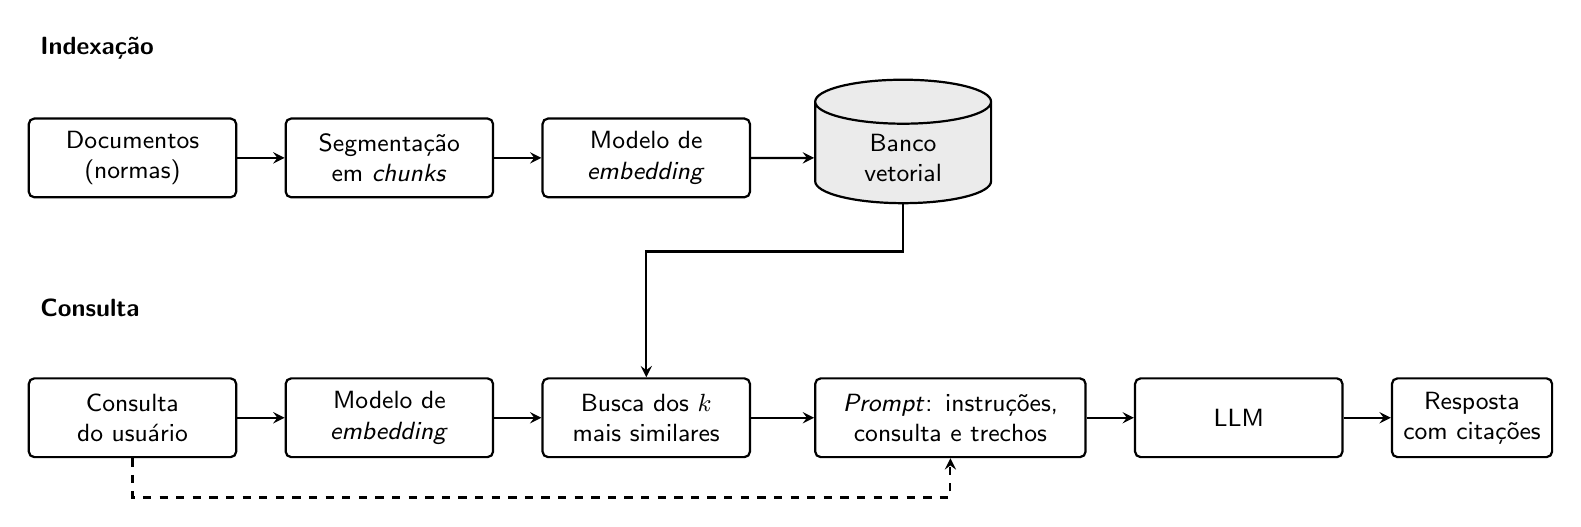
\begin{tikzpicture}[
		font=\small,
		caixa/.style={draw, rounded corners=2pt, align=center, minimum height=10mm, text width=24mm, fill=white},
		banco/.style={draw, cylinder, shape border rotate=90, aspect=0.25, align=center, minimum height=14mm, text width=20mm, fill=black!8},
		>=stealth, every path/.style={->, thick}]
		% indexação
		\node[font=\small\bfseries, anchor=west] at (-1.3,1.4) {Indexação};
		\node[caixa] (docs) at (0,0) {Documentos\\(normas)};
		\node[caixa, right=6mm of docs] (chunk) {Segmentação\\em \textit{chunks}};
		\node[caixa, right=6mm of chunk] (emb1) {Modelo de\\\textit{embedding}};
		\node[banco, right=8mm of emb1] (vdb) {Banco\\vetorial};
		\draw (docs) -- (chunk);
		\draw (chunk) -- (emb1);
		\draw (emb1) -- (vdb);
		% consulta
		\node[font=\small\bfseries, anchor=west] at (-1.3,-1.9) {Consulta};
		\node[caixa] (q) at (0,-3.3) {Consulta\\do usuário};
		\node[caixa, right=6mm of q] (emb2) {Modelo de\\\textit{embedding}};
		\node[caixa, right=6mm of emb2] (busca) {Busca dos $k$\\mais similares};
		\node[caixa, right=8mm of busca, text width=32mm] (prompt) {\textit{Prompt}: instruções,\\consulta e trechos};
		\node[caixa, right=6mm of prompt] (llm) {LLM};
		\node[caixa, right=6mm of llm, text width=18mm] (resp) {Resposta\\com citações};
		\draw (q) -- (emb2);
		\draw (emb2) -- (busca);
		\draw (vdb.south) |- ++(0,-6mm) -| (busca.north);
		\draw (busca) -- (prompt);
		\draw (prompt) -- (llm);
		\draw (llm) -- (resp);
		\draw[dashed] (q.south) -- ++(0,-5mm) -| (prompt.south);
	\end{tikzpicture}}
	\fonte{Elaborado pelo autor, com base em \citeonline{Lewis2020} e \citeonline{Gao2023}.}
\end{figure}

Como o conhecimento fica fora do modelo, atualizar o sistema é reindexar documentos, sem retreinar nada: quando uma portaria é alterada, basta indexar o texto consolidado. E como cada trecho recuperado carrega sua origem, pode-se pedir ao modelo que cite a fonte de cada afirmação, o que permite ao usuário conferir a resposta no documento original. Essas duas propriedades, atualização e rastreabilidade, tornam o RAG adequado a sistemas governamentais \cite{Montero2025,Montero2026}.

\subsection{Paradigmas e variações}

\citeonline{Gao2023} organizam a evolução dos sistemas RAG em três paradigmas. O \textbf{RAG ingênuo} segue apenas o fluxo de indexar, recuperar e gerar descrito acima. O \textbf{RAG avançado} acrescenta etapas antes e depois da recuperação. Antes, a consulta pode ser reescrita, expandida com sinônimos e siglas ou decomposta em subconsultas; depois, os trechos recuperados podem ser reordenados por um modelo de reranqueamento, em geral um codificador cruzado (Seção~\ref{sec:embedding}), ou comprimidos, para que só o conteúdo mais relevante chegue ao LLM. O \textbf{RAG modular} trata o sistema como um conjunto de módulos combináveis, como buscas híbridas, recuperação iterativa e roteamento entre bases, e inclui as arquiteturas em que agentes decidem quando e o que recuperar.

Outra decisão de projeto é a origem da consulta. Em assistentes de perguntas e respostas, a consulta é a própria pergunta do usuário. Em tarefas de análise de processos, como as tratadas neste trabalho, não há uma pergunta: a consulta precisa ser construída a partir da tarefa ou do conteúdo do processo. Uma consulta fixa, igual para todos os processos, recupera sempre os mesmos trechos, enquanto consultas derivadas dos documentos de cada processo fazem o contexto acompanhar o caso. O Capítulo~\ref{cap:metodologia} descreve como o DocFlow constrói essas consultas.

\subsection{Limitações e avaliação}

O RAG transfere parte do problema para a recuperação. Se os trechos relevantes não forem recuperados, o modelo responde sem eles ou com trechos irrelevantes, que podem desviá-lo. Na PDSA-RS, a maior parte das falhas do sistema RAG veio de erros de recuperação \cite{Montero2025}. Mesmo quando os trechos certos são recuperados, nada garante que o modelo os use corretamente: o contexto pode ser longo, com a informação relevante no meio \cite{Liu2024}, ou a norma pode não conter o critério de que a decisão depende.

Por isso, a avaliação de sistemas RAG costuma separar os dois componentes. A recuperação é avaliada com métricas da área de recuperação de informação, como a revocação nos $k$ primeiros resultados (Recall@$k$), que mede se os trechos relevantes estão entre os recuperados \cite{Manning2008}. A geração é avaliada pela correção da resposta em relação a um gabarito ou por critérios como a fidelidade da resposta ao contexto recuperado e sua relevância para a pergunta, que podem ser estimados automaticamente com o auxílio de um LLM, como no \textit{framework} RAGAS \cite{Es2024}. Em tarefas de decisão, como a deste trabalho, a referência mais direta é a decisão tomada pelos especialistas humanos no mesmo processo.

% ------------------------------------------------------------
\section{PDSA-RS e Trabalhos Anteriores}
\label{sec:pdsa}

Este trabalho dá continuidade a uma linha de pesquisa do LUMAC sobre o uso de LLMs e RAG em plataformas governamentais de defesa sanitária, iniciada na Plataforma de Defesa Sanitária Animal do Rio Grande do Sul (PDSA-RS). Criada em 2019, a PDSA-RS apoia a sanidade e a produção animal no estado por meio de uma plataforma digital para a gestão de certificações e o acompanhamento da conformidade sanitária \cite{Montero2025}. Foi desenvolvida pela UFSM em parceria com o Ministério da Agricultura e Pecuária (MAPA), com apoio do Fundo de Desenvolvimento e Defesa Sanitária Animal (FUNDESA), e integra as etapas da certificação de estabelecimentos avícolas e suínos, ligando inspeções veterinárias, laboratórios e autoridades de defesa agropecuária. Produtores e fiscais acompanham pela plataforma os exames sanitários, o processamento das amostras e a emissão dos certificados exigidos para a movimentação de animais no país e no exterior \cite{Montero2025}. A plataforma adota uma arquitetura orientada a microsserviços, com portais para cada público, como o Serviço Veterinário Estadual, os responsáveis técnicos, os laboratórios e o MAPA \cite{Montero2025}.

Sobre essa plataforma, o grupo aplicou RAG pela primeira vez no módulo de certificação avícola: as instruções normativas que definem os exames exigidos foram indexadas, e um LLM pequeno, executado localmente, passou a responder sobre a condição sanitária das solicitações, com acurácia de 55\% contra 12\% do mesmo modelo sem recuperação \cite{Montero2025iceis,Montero2025}. Em seguida, \citeonline{Montero2026} propuseram uma arquitetura genérica de assistente para analistas do setor público e avaliaram seu motor de geração em pareceres sobre recursos administrativos julgados pela JAP da SEAPI-RS. Essa arquitetura foi depois implementada como a plataforma DocFlow, descrita no Capítulo~\ref{cap:metodologia}. Esses trabalhos são analisados em detalhe na Seção~\ref{sec:tr-grupo}.

% ------------------------------------------------------------
\section{PNIP e a Certificação Higiênico-Sanitária}
\label{sec:pnip}

\subsection{A Plataforma Nacional da Indústria do Pescado}

A Plataforma Nacional da Indústria do Pescado (PNIP), instituída pela Portaria MPA nº~361/2024 \cite{MPA2024}, é a plataforma digital oficial do Ministério da Pesca e Aquicultura para o envio, a análise e a emissão das certificações do setor pesqueiro.
Ao centralizar esses fluxos, a plataforma apoia a rastreabilidade que liga cada produto pesqueiro à sua origem legal \cite{Olsen2018}, um dos pilares do combate à pesca ilegal, não declarada e não regulamentada, que responde por uma parcela relevante das capturas mundiais \cite{Agnew2009}.

Cada solicitação é analisada por perfis hierárquicos (analista técnico, coordenador e diretor), o que exige conhecimento aprofundado de normas que mudam com o tempo. A plataforma também se integra a sistemas externos do governo e de parceiros, como SERPRO, CRMV, SISRGP, PesqBrasil e SEI, para validar dados e tramitar documentos.

\subsection{A certificação higiênico-sanitária de embarcações}

A certificação higiênico-sanitária de embarcações pesqueiras é regida pela Portaria SAP/MAPA nº~310/2020, alterada pelas Portarias MPA nº~171/2023 e nº~742/2026 \cite{Portaria310,Portaria171,Portaria742}, e resulta no Certificado Oficial de Boas Práticas Higiênico-Sanitárias a Bordo, válido por cinco anos. A norma estabelece os requisitos que a embarcação deve cumprir, como o programa de autocontrole, a potabilidade da água usada a bordo, o treinamento da tripulação, o controle de pragas e as características do material de revestimento das áreas em contato com o pescado, e traz no Anexo~I a lista de verificação usada na análise. A Portaria 742/2026 acrescentou requisitos específicos para a secagem de bexiga natatória e o congelamento de camarão e lagostim a bordo.

Para solicitar o certificado, o técnico responsável pela embarcação preenche na PNIP a lista de verificação do Anexo~I e anexa as evidências de cada requisito, organizadas por categoria:

\begin{itemize}
	\item programa de autocontrole (PAC) e registros de controle a bordo;
	\item registros de treinamento da tripulação;
	\item documentos do controle de pragas;
	\item laudo de potabilidade da água e declaração do fornecedor de água;
	\item documento do material de revestimento;
	\item declaração de responsabilidade;
	\item registros fotográficos datados da embarcação e de seus equipamentos;
	\item outros documentos.
\end{itemize}

\subsection{A análise técnica e o parecer}

O analista verifica cada item da lista de verificação contra os anexos, registra as não conformidades e redige um parecer técnico, que avalia os dados da embarcação, cada categoria de documentos e cada item da lista e conclui de forma favorável ou desfavorável. Se faltar algum item ou a evidência for insuficiente, o analista solicita complementos, e o técnico tem 30 dias corridos para apresentá-los; caso contrário, a solicitação é indeferida. A decisão depende, portanto, de o conteúdo de cada anexo comprovar o requisito correspondente, e não apenas de o anexo existir. Nos registros fotográficos, por exemplo, o analista verifica se o conjunto de fotos cobre as vistas exigidas da embarcação e se as fotos pertencem a ela.

É esse julgamento que este trabalho procura apoiar. Em comparação com a certificação avícola da PDSA-RS, em que a decisão decorre de dados estruturados de exames laboratoriais, a certificação HS envolve documentos heterogêneos, muitas vezes digitalizados, e dezenas de fotografias por processo, e cabe ao analista julgar se a evidência é suficiente. A revisão apresentada no Capítulo~\ref{cap:trabalhos-relacionados} não encontrou estudos que combinassem os documentos de um dossiê, seus registros fotográficos e as normas recuperadas para apoiar esse tipo de julgamento.

% Capítulos previstos (arquivos ainda não criados):
% % ============================================================
% Capítulo 3 - Trabalhos Relacionados
% Base: artigos do grupo em artigo-iceis-guedes/artigos-iceis/ (Montero2025iceis,
% Montero2025, Montero2026) e a RSL (artigo-iceis-guedes/rsl.tex, RSL-Rayyan/).
% Versão anterior, com o protocolo completo da RSL e o fluxo PRISMA, no histórico do git
% (commit 4958c4d), caso a banca peça o detalhamento.
% ============================================================
\chapter{Trabalhos Relacionados}
\label{cap:trabalhos-relacionados}

Este capítulo apresenta os trabalhos mais próximos deste. A Seção~\ref{sec:tr-grupo} analisa os trabalhos anteriores do grupo, dos quais este é continuação direta: o RAG na certificação avícola da PDSA-RS e a arquitetura de assistente para analistas proposta por \citeonline{Montero2026}, que deu origem ao DocFlow. A Seção~\ref{sec:rsl} resume uma revisão sistemática rápida sobre LLMs e RAG na administração pública, feita para situar o trabalho na literatura mais ampla, e a Seção~\ref{sec:tr-lacuna} compara este trabalho com os estudos mais próximos.

% ------------------------------------------------------------
\section{Trabalhos Anteriores do Grupo}
\label{sec:tr-grupo}

A Seção~\ref{sec:pdsa} apresentou a PDSA-RS e o contexto em que esses trabalhos surgiram. Esta seção os examina com mais detalhe, com atenção às escolhas de projeto, à forma de avaliação e às limitações apontadas pelos próprios autores, porque são elas que orientaram as decisões deste trabalho.

\subsection{RAG na certificação sanitária avícola}

O primeiro trabalho integrou um sistema RAG ao módulo de certificação avícola da PDSA-RS \cite{Montero2025iceis}, e sua versão estendida detalha a implementação e a avaliação \cite{Montero2025}. A base de conhecimento reúne as Instruções Normativas nº~44/2001 e nº~78/2003, que definem os exames exigidos conforme a idade das aves e a finalidade da produção. Os textos foram indexados com o LlamaIndex em trechos de 1.024 caracteres com sobreposição de 200, isto é, por tamanho fixo e não pela estrutura da norma (Seção~\ref{sec:chunking}). Os \textit{embeddings} foram gerados com o \texttt{bge-large-en-v1.5} e armazenados no PostgreSQL com o pgvector, e a geração usou o LLaMA 3.1 8B Instruct, executado localmente pelo Ollama com temperatura 0,4, para que os dados dos produtores não saíssem da infraestrutura da universidade. Além das normas, a base passou a receber relatórios em linguagem natural gerados a partir dos dados estruturados de cada solicitação, como os resultados dos exames, de modo que a recuperação pudesse trazer tanto o requisito quanto a evidência do caso. A consulta é disparada por um botão na tela de análise e atendida por um \textit{endpoint} da API de certificação avícola \cite{Montero2025}.

A avaliação usou 100 solicitações sorteadas da plataforma, o que, segundo os autores, corresponde a cerca de um terço das solicitações enviadas pelos pouco mais de 300 estabelecimentos de genética avícola do estado. Um especialista do domínio classificou cada resposta como correta, parcialmente correta ou incorreta. O modelo sem recuperação acertou 12 das 100; com RAG, foram 55 respostas corretas, 20 parcialmente corretas e 25 incorretas. Das 25 incorretas, 15 vieram de erros de recuperação, em que o sistema trouxe trechos genéricos ou conflitantes em vez da cláusula exigida, e 10 de falhas de síntese, em que o modelo não chegou à conclusão certa mesmo com o contexto correto \cite{Montero2025}. Os próprios autores apontam como limitações o domínio único, a dependência da qualidade da recuperação e a persistência de alucinações, que torna indispensável a revisão do analista.

Três características desse trabalho importam para a comparação com a PNIP. A decisão decorre da aplicação da norma a dados estruturados (quais exames foram feitos, em que idade e com que resultado), de modo que, recuperado o requisito certo, a resposta correta é em grande parte determinada. A segmentação por tamanho fixo e a principal causa de erro, a recuperação, motivaram a segmentação por artigo adotada depois pelo grupo e neste trabalho. E a referência da avaliação foi o julgamento de um especialista sobre cada resposta, e não a decisão registrada no processo.

\subsection{Pareceres em recursos administrativos}

Em seguida, \citeonline{Montero2026} passaram de perguntas sobre requisitos à redação de pareceres. O trabalho propõe uma arquitetura de assistente para analistas do setor público, concebida como um módulo integrado ao sistema legado do órgão por meio de um \textit{gateway} de API, para que o assistente funcione dentro da interface que o analista já usa. A arquitetura tem quatro pilares:

\begin{itemize}
	\item um \textit{pipeline} multimodal, que converte tudo em texto: OCR para documentos digitalizados, um modelo de imagem para texto para as fotos e um modelo de fala para texto para os áudios;
	\item um núcleo de raciocínio baseado em RAG, com a legislação segmentada no nível dos artigos e recuperada por similaridade de cosseno a partir dos argumentos do caso;
	\item uma camada de governança de dados alinhada à LGPD, que remove dados pessoais com expressões regulares, para dados estruturados como o CPF, e com reconhecimento de entidades nomeadas baseado no BERTimbau, para nomes e outros dados não estruturados;
	\item uma etapa de revisão humana, em que o analista revisa os resumos da infração e da defesa gerados pelo modelo antes de eles serem usados na redação da minuta.
\end{itemize}

Os autores deixam claro que essa arquitetura era conceitual e não havia sido implementada; o trabalho avaliou apenas o seu motor de geração \cite{Montero2026}. O experimento usou 14 recursos administrativos reais da Junta Administrativa de Recursos de Infrações (JAP) da SEAPI-RS \verificar{o nome oficial da JAP}, escolhidos por um especialista do órgão para cobrir casos simples e complexos, dos quais 11 tiveram o auto de infração mantido e 3 anulado. Os documentos de cada processo (auto de infração, evidências externas e defesa) foram transcritos manualmente para texto. O modelo foi o Gemini 2.5 Pro, e a recuperação foi \textit{simulada}: o texto integral da Lei estadual nº~13.467/2010 e do Decreto nº~52.434/2015 foi colocado no \textit{prompt}, para isolar a capacidade de raciocínio do modelo de eventuais erros de recuperação. A geração seguiu duas etapas, uma análise detalhada seguida da redação do parecer no modelo oficial da JAP, e foi repetida com temperaturas de 0,5, 1,0 e 1,5, com \textit{top-p} fixo em 0,8, totalizando 42 pareceres.

As decisões foram as mesmas nas três temperaturas: 71,4\% de acurácia, $\kappa$ de Cohen de 0,317 e dois dos três recursos providos identificados. Os autores observam que essa acurácia fica abaixo dos 78,6\% de uma regra que mantém todos os autos, mas que essa regra não identificaria nenhum auto a anular, o que o $\kappa$ e a sensibilidade na classe minoritária capturam. Os pareceres tiveram similaridade de cosseno acima de 0,90 e BERTScore F1 entre 0,70 e 0,85 em relação aos pareceres humanos. A análise qualitativa, guiada por uma lista de nove perguntas, foi a mais reveladora: no caso de maior erro, a defesa se apoiava em uma lei já revogada, e o modelo aceitou o argumento mesmo tendo a legislação vigente no contexto; em outros casos, não reproduziu o raciocínio espaço-temporal do analista ou divergiu dele na aplicação da proporcionalidade da pena. Temperaturas menores produziram textos mais concisos e formais \cite{Montero2026}. Como limitações, os autores citam a amostra de 14 casos de um único órgão, a recuperação simulada, a avaliação de um único modelo, a falta de comparação direta com linhas de base e a ausência de avaliação da implantação.

\subsection{Do assistente proposto a este trabalho}

A arquitetura de \citeonline{Montero2026} foi depois implementada pelo seu primeiro autor como a plataforma DocFlow (Capítulo~\ref{cap:metodologia}), com mudanças em relação ao projeto original: um monólito modular em vez de serviços atrás de um \textit{gateway}, LLMs multimodais que recebem as imagens diretamente em vez de um modelo que as descreve em texto, e a revisão humana como contrato da API. Em paralelo, o grupo também propôs uma arquitetura que combina raciocínio baseado em casos e LLMs para a certificação de produtos pesqueiros \cite{Casanova2026}.

Este trabalho aplica o DocFlow à PNIP e responde a várias das continuações apontadas por \citeonline{Montero2026}: a recuperação deixa de ser simulada e é implementada e medida, com segmentação por artigo e consultas derivadas de cada processo; a avaliação usa mais processos (40), vários modelos, abertos e hospedados, e linhas de base explícitas, como o acaso e uma regra baseada em categorias de documento ausentes; e a plataforma é avaliada de ponta a ponta sobre dossiês reais, sem transcrição manual. A Tabela~\ref{tab:tr-grupo} resume as diferenças.

\begin{table}[htb]
	\centering
	\caption{Comparação entre os trabalhos anteriores do grupo e este trabalho.}
	\label{tab:tr-grupo}
	\footnotesize
	\setlength{\tabcolsep}{3pt}
	\begin{tabular}{|L{0.17\textwidth}|L{0.24\textwidth}|L{0.24\textwidth}|L{0.24\textwidth}|}
		\hline
		& \textbf{\citeonline{Montero2025}} & \textbf{\citeonline{Montero2026}} & \textbf{Este trabalho} \\
		\hline
		Processo & Certificação avícola (PDSA-RS) & Recursos de infrações (JAP/SEAPI-RS) & Certificação HS de embarcações (PNIP) \\
		\hline
		Tarefa & Verificar a condição sanitária de solicitações & Redigir parecer e decidir & Sugerir decisão e redigir parecer \\
		\hline
		Evidência & Dados estruturados de exames, convertidos em relatórios & Documentos transcritos manualmente & Dossiês com documentos digitalizados (OCR) e fotografias \\
		\hline
		Segmentação & Tamanho fixo (1.024 caracteres) & Por artigo (proposta) & Por artigo \\
		\hline
		Recuperação & RAG a partir de uma pergunta sobre a solicitação & Simulada (normas inteiras no \textit{prompt}) & RAG com consulta fixa e consultas por processo; norma inteira como controle \\
		\hline
		Imagens & Não & Previstas, convertidas em texto & Enviadas ao modelo como imagens \\
		\hline
		Modelos & LLaMA 3.1 8B (local) & Gemini 2.5 Pro (hospedado) & Gemma 4 e Qwen3-VL (locais); GPT-6 Luna, Gemini 3.5 Flash-Lite e Claude Haiku 5.5 (hospedados) \\
		\hline
		Amostra & 100 solicitações & 14 recursos & 40 processos (20 nos rascunhos) \\
		\hline
		Referência & Julgamento de especialista sobre cada resposta & Decisões e pareceres dos analistas & Decisões e pareceres dos analistas \\
		\hline
		Resultado principal & RAG elevou a acurácia de 12\% para 55\% & 71,4\% de acurácia, $\kappa=0{,}317$ & Decisões no nível do acaso; recuperação por processo melhor que a fixa \\
		\hline
	\end{tabular}
	\fonte{Elaborado pelo autor, a partir de \citeonline{Montero2025}, \citeonline{Montero2026} e do Capítulo~\ref{cap:estudo-caso}.}
\end{table}

A diferença mais importante, porém, está na natureza da decisão. Na certificação avícola, a resposta decorre de regras aplicadas a dados estruturados; nos recursos da JAP, de argumentos jurídicos confrontados com a legislação; na certificação HS, de um julgamento sobre se o conteúdo de documentos heterogêneos e de dezenas de fotografias é evidência suficiente de cada requisito. Se os ganhos obtidos nos dois primeiros cenários se transferem para o terceiro é a pergunta que este trabalho investiga (Seção~\ref{sec:problema}).

% ------------------------------------------------------------
\section{Revisão Sistemática Rápida}
\label{sec:rsl}

Para situar este trabalho além do grupo, foi conduzida, em conjunto com o coautor do artigo que lhe deu origem, uma revisão sistemática rápida sobre o uso de LLMs e RAG na administração pública. Revisões rápidas seguem as etapas de uma revisão sistemática, mas simplificam algumas delas; aqui, a elegibilidade foi avaliada em uma única etapa de triagem. A revisão buscou responder como LLMs e RAG estão sendo aplicados no setor público (QP1), que tarefas administrativas apoiam (QP2) e como são avaliados e que desafios são relatados (QP3).

As buscas foram feitas em 8 de novembro de 2026 na Scopus, na Web of Science, na IEEE Xplore e na ACM Digital Library, com uma \textit{string} que combinou termos de LLM e RAG, no título ou no resumo; termos do setor público, apenas no título, incluindo segurança dos alimentos e inspeção sanitária, para captar o domínio da PNIP; e termos ligados a documentos, normas e inspeções. Foram considerados artigos de periódico e de conferência de 2020 a 2026, em inglês ou português. As buscas retornaram 290 registros, dos quais o Rayyan removeu 181 duplicatas \verificar{uma deduplicação preliminar por DOI e título havia estimado 119 duplicatas; conferir no Rayyan}. Os dois revisores triaram os 109 registros restantes pelo título e pelo resumo, de forma independente e cega, e concordaram em 96 deles ($\kappa$ de Cohen \cite{Cohen1960} de 0,69 com as três categorias de decisão e de 0,88 entre incluir e não incluir); os conflitos foram resolvidos por consenso. Foram incluídos 86 estudos, classificados conforme a Tabela~\ref{tab:rsl}.

\begin{table}[htb]
	\centering
	\caption{Classificação dos 86 estudos incluídos na revisão.}
	\label{tab:rsl}
	\small
	\begin{tabular}{|l|r|r|}
		\hline
		\textbf{Categoria} & \textbf{n} & \textbf{\%} \\
		\hline
		\multicolumn{3}{|l|}{\textit{Arquitetura}} \\
		\hline
		LLM sem recuperação externa & 38 & 44 \\
		RAG ou variante com recuperação & 31 & 36 \\
		Sem sistema (sobretudo estudos de adoção) & 17 & 20 \\
		\hline
		\multicolumn{3}{|l|}{\textit{Tarefa apoiada (um estudo pode ter mais de uma)}} \\
		\hline
		Análise de documentos & 38 & 44 \\
		Serviços ao cidadão e perguntas e respostas & 29 & 34 \\
		Conformidade regulatória & 15 & 17 \\
		Pareceres técnicos e decisões & 7 & 8 \\
		Domínio sanitário e alimentar & 7 & 8 \\
		Compras públicas & 6 & 7 \\
		\hline
	\end{tabular}
	\fonte{Elaborado pelo autor.}
\end{table}

O tema é recente: nenhum estudo incluído é anterior a 2024, e 48 são de 2026. Quanto às aplicações (QP1), o RAG já aparece em mais de um terço dos estudos, em geral para embasar as respostas em normas e documentos oficiais, às vezes com grafos de conhecimento \cite{Zeng2026,Papageorgiou2025} ou com vários agentes, como no DataGovAI, que apoia servidores de Utah, nos Estados Unidos, na aplicação de regras de retenção de dados \cite{Memari2026}. A soberania dos dados leva a implantações locais \cite{Ayuyang2026}, a modelos de código aberto \cite{Mala2025} e a treinamento federado \cite{JimenezGutierrez2026}, preocupação que também orientou os trabalhos do grupo. A segmentação dos textos legais é recorrente: o tamanho e a estrutura dos trechos afetam a recuperação \cite{Boonmee2026,Kawashima2024}, e em normas indonésias a divisão nos limites dos artigos atingiu 90\% de acurácia nas respostas \cite{Fiddina2026}.

Quanto às tarefas (QP2), predominam a análise de documentos (44\%), como perguntas sobre normas \cite{Fiddina2026,Legado2026} e a revisão das descrições de serviços do Gov.br \cite{Ramos2025}, e os assistentes ao cidadão (34\%). Apenas 7 estudos (8\%) apoiam pareceres ou decisões, a tarefa mais próxima da deste trabalho, entre eles a avaliação de propostas em licitações \cite{Sofat2024,Zeng2026}, a avaliação de estudos de viabilidade de projetos de investimento, em que os LLMs se saíram melhor em critérios explícitos do que nos que exigem julgamento \cite{Sheng2026}, e o próprio trabalho do grupo na JAP \cite{Montero2026}.

Quanto à avaliação (QP3), as práticas são heterogêneas: métricas de recuperação como Recall@$k$ e MRR \cite{Boonmee2026,Liu2025}, acurácia ou métricas do RAGAS para as respostas \cite{Fiddina2026,Memari2026} e \textit{benchmarks} que mostram baixa robustez a pequenas variações na entrada \cite{Liu2025b}. Poucos estudos medem o efeito sobre o trabalho dos servidores: em um governo local, um sistema RAG manteve a acurácia dos servidores em perguntas curtas e reduziu seu tempo de trabalho em 23,6\%, mas foi pior em perguntas descritivas \cite{Kawashima2024}. Os desafios mais citados são a privacidade, as alucinações e a confiança nas respostas, e os estudos qualitativos acrescentam que a responsabilização se dilui quando os servidores adotam as saídas por padrão \cite{Jonathan2026}, que os servidores esperam ajuda em subtarefas e não a automação da decisão \cite{Drobotowicz2026} e que as organizações públicas brasileiras ainda carecem de governança para o uso da IA generativa \cite{Alves2024,Canedo2026}. Esses resultados reforçam a escolha de manter o analista como responsável pela decisão.

Os sete estudos do domínio sanitário e alimentar tratam da fiscalização e da regulação, e não da análise de solicitações: um modelo especializado em segurança dos alimentos obtido por \textit{fine-tuning} \cite{Shen2026}, a extração de informações de normas \cite{Zhao2026}, a sumarização de documentos \cite{Bakagianni2025}, o planejamento de inspeções \cite{Yu2026} e a avaliação, com LLMs visuais, da infraestrutura de vendedores de comida de rua a partir de vídeos \cite{Chernikov2025}, o único estudo incluído que usa imagens como evidência de conformidade sanitária.

% ------------------------------------------------------------
\section{Comparação e Lacuna}
\label{sec:tr-lacuna}

A Tabela~\ref{tab:rsl-comparacao} compara este trabalho com os estudos da revisão mais próximos dele; os trabalhos do grupo já foram comparados na Tabela~\ref{tab:tr-grupo}. Nenhum dos estudos incluídos gera pareceres técnicos sobre solicitações de certificação combinando os documentos de um dossiê, seus registros fotográficos e a recuperação das normas aplicáveis. Além dos trabalhos do grupo, que trataram de processos estaduais de sanidade animal sem evidências fotográficas, nenhum aplica RAG a pareceres no domínio sanitário. Este trabalho ocupa essa lacuna na certificação federal de embarcações pesqueiras da PNIP, medindo o efeito do contexto normativo recuperado e das fotos e tomando como referência as decisões e os pareceres dos analistas.

\begin{table}[htb]
	\centering
	\caption{Comparação entre este trabalho e os estudos mais próximos encontrados na revisão.}
	\label{tab:rsl-comparacao}
	\footnotesize
	\setlength{\tabcolsep}{3pt}
	\begin{tabular}{|L{0.16\textwidth}|L{0.2\textwidth}|L{0.18\textwidth}|L{0.13\textwidth}|L{0.08\textwidth}|L{0.16\textwidth}|}
		\hline
		\textbf{Trabalho} & \textbf{Domínio} & \textbf{Tarefa} & \textbf{Recuperação} & \textbf{Imagens} & \textbf{Referência} \\
		\hline
		\citeonline{Fiddina2026} & Normas governamentais (Indonésia) & Perguntas e respostas & RAG por artigo & Não & Gabarito de perguntas e respostas \\
		\hline
		\citeonline{Memari2026} & Retenção de dados (Utah, EUA) & Conformidade & RAG multiagente & Não & Consultas sintéticas (RAGAS) \\
		\hline
		\citeonline{Sheng2026} & Projetos de investimento (China) \verificar{país} & Avaliar estudos de viabilidade & Não descrita & Não & Notas de especialistas \\
		\hline
		\citeonline{Shen2026} & Segurança dos alimentos & Várias (\textit{benchmark}) & Não (\textit{fine-tuning}) & Não & \textit{Benchmark} de 10 tarefas \\
		\hline
		\citeonline{Chernikov2025} & Comida de rua (Índia) & Avaliar infraestrutura & Não descrita & Sim (vídeo) & Questionário de campo \\
		\hline
		\textbf{Este trabalho} & Certificação HS de embarcações (PNIP) & Sugerir decisão e redigir parecer & RAG por artigo, consultas por processo & Sim (fotos) & Decisões e pareceres dos analistas \\
		\hline
	\end{tabular}
	\fonte{Elaborado pelo autor.}
\end{table}
   % RSL: fora até decidir se entra no TCC II
% % ============================================================
% Capítulo 4 - Metodologia (a plataforma DocFlow e as extensões para a PNIP)
% Base: artigo ICEIS (artigo-iceis-guedes/main.tex), Seção 3 (versão de 16/11/2026).
% ============================================================
\chapter{Metodologia}
\label{cap:metodologia}

Este capítulo descreve a plataforma DocFlow e as extensões feitas nela para a certificação HS da PNIP. O DocFlow transforma em plataforma implementada a arquitetura de assistente para analistas do setor público proposta por \citeonline{Montero2026}, que era conceitual (Seção~\ref{sec:tr-grupo}). Três mudanças de projeto se destacam. Os serviços atrás de um \textit{gateway} de API deram lugar a um monólito modular (Seção~\ref{sec:principios}). O modelo de visão separado deu lugar a LLMs multimodais, que recebem as imagens diretamente (Seção~\ref{sec:execucao}). E a revisão humana, que era uma etapa do fluxo, tornou-se um contrato da API: toda tarefa nasce pendente de revisão, o conteúdo gerado é imutável e toda transição é auditada (Seção~\ref{sec:revisao-humana}). Como o DocFlow foi implementado pelo primeiro autor de \citeonline{Montero2026}, a contribuição deste trabalho está nas extensões descritas nas Seções~\ref{sec:base-conhecimento} e~\ref{sec:execucao} e na sua avaliação na PNIP, relatada no Capítulo~\ref{cap:estudo-caso}.

% ------------------------------------------------------------
\section{Princípios de projeto}
\label{sec:principios}

O DocFlow é um monólito modular escrito em Java~21 com Spring Boot 3.3.5 e Spring AI 1.0, organizado segundo a arquitetura hexagonal (portas e adaptadores). Nessa arquitetura, o domínio e os casos de uso ficam no centro e dependem apenas de interfaces, as portas; o acesso a bancos de dados, a serviços externos e aos provedores de LLM é feito por adaptadores que implementam essas portas. O projeto segue cinco princípios:

\begin{itemize}
	\item \textbf{revisão humana por construção}: a plataforma nunca produz uma decisão final (Seção~\ref{sec:revisao-humana});
	\item \textbf{independência de domínio}: um novo domínio, como a certificação HS, é configuração, e não código;
	\item \textbf{neutralidade de provedor}: OpenAI, Anthropic, Gemini, Ollama e vLLM ficam atrás de uma mesma porta;
	\item \textbf{privacidade desde a concepção}: dados pessoais detectáveis são removidos do texto antes de ele chegar a um LLM;
	\item \textbf{auditabilidade}: execuções, \textit{prompts}, revisões e acessos são registrados.
\end{itemize}

A Figura~\ref{fig:arquitetura} mostra os principais componentes. À esquerda ficam os adaptadores que acionam a plataforma (a API REST, com autenticação e papéis, e um SDK para clientes), usados pelo sistema hospedeiro, como a PNIP; à direita, os adaptadores acionados por ela: extração de texto, OCR e remoção de dados pessoais, armazenamento de objetos (arquivos e fotos), banco vetorial, modelos de \textit{embedding} e provedores de LLM. Como o domínio depende apenas de suas portas, regra verificada por testes de arquitetura com o ArchUnit, trocar o provedor de LLM não altera o domínio. Foi isso que permitiu executar localmente, pelo Ollama, o modelo de \textit{embedding} e os modelos abertos de geração, e acessar os modelos hospedados por suas APIs, sem mudar o restante da plataforma.

\begin{figure}[htb]
	\centering
	\caption{O DocFlow como um hexágono: os adaptadores à esquerda acionam as portas de entrada, e os adaptadores à direita implementam as portas de saída. Todas as dependências apontam para dentro.}
	\label{fig:arquitetura}
	\resizebox{\textwidth}{!}{%
	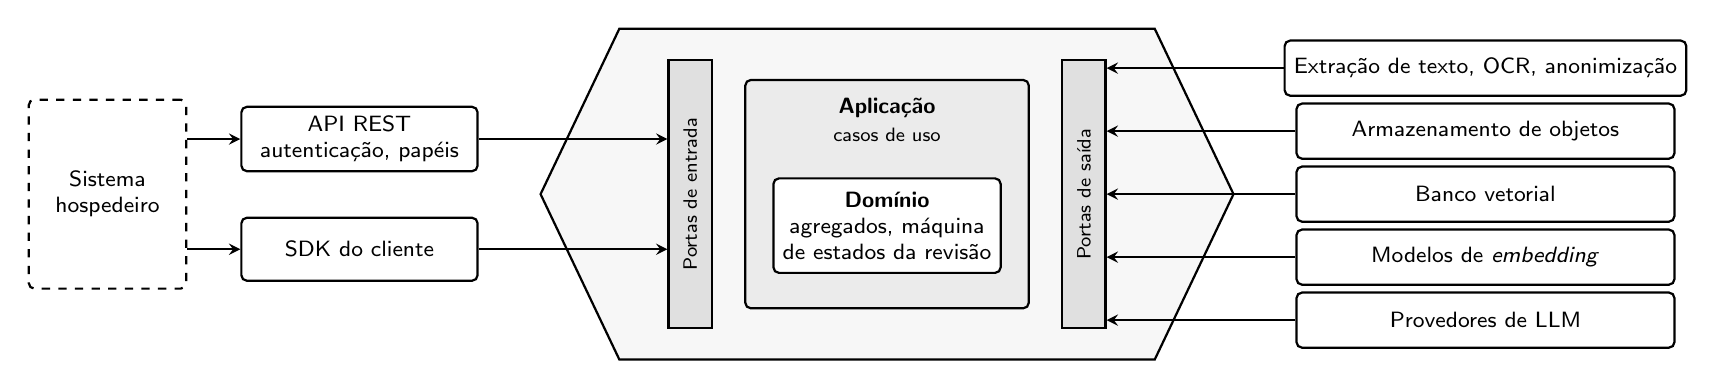
\begin{tikzpicture}[
		font=\footnotesize,
		box/.style={draw, rounded corners=2pt, align=center, minimum height=8mm, fill=white},
		port/.style={draw, minimum width=5.5mm, minimum height=48mm, fill=black!12, font=\scriptsize},
		>=stealth, every path/.style={->, thick}]
		\draw[-, thick, fill=black!3] (-4.4,0) -- (-3.4,2.1) -- (3.4,2.1) -- (4.4,0) -- (3.4,-2.1) -- (-3.4,-2.1) -- cycle;
		\node[box, minimum width=36mm, minimum height=29mm, fill=black!8] (app) at (0,0) {};
		\node[font=\footnotesize\bfseries] at (0,1.1) {Aplicação};
		\node[font=\scriptsize] at (0,0.75) {casos de uso};
		\node[box, minimum width=28mm, minimum height=12mm] at (0,-0.4) {\textbf{Domínio}\\agregados, máquina\\de estados da revisão};
		\node[port, minimum height=34mm] (pin) at (-2.5,0) {\rotatebox{90}{Portas de entrada}};
		\node[port, minimum height=34mm] (pout) at (2.5,0) {\rotatebox{90}{Portas de saída}};
		\node[box, minimum width=30mm] (rest) at (-6.7,0.7) {API REST\\autenticação, papéis};
		\node[box, minimum width=30mm] (sdk) at (-6.7,-0.7) {SDK do cliente};
		\node[box, minimum width=20mm, minimum height=24mm, dashed] (host) at (-9.9,0) {Sistema\\hospedeiro};
		\node[box, minimum width=48mm, minimum height=7mm] (ext) at (7.6,1.6) {Extração de texto, OCR, anonimização};
		\node[box, minimum width=48mm, minimum height=7mm] (obj) at (7.6,0.8) {Armazenamento de objetos};
		\node[box, minimum width=48mm, minimum height=7mm] (vec) at (7.6,0.0) {Banco vetorial};
		\node[box, minimum width=48mm, minimum height=7mm] (emb) at (7.6,-0.8) {Modelos de \textit{embedding}};
		\node[box, minimum width=48mm, minimum height=7mm] (llm) at (7.6,-1.6) {Provedores de LLM};
		\draw (host.east |- rest.west) -- (rest.west);
		\draw (host.east |- sdk.west) -- (sdk.west);
		\draw (rest.east) -- (pin.west |- rest.east);
		\draw (sdk.east) -- (pin.west |- sdk.east);
		\foreach \n in {ext,obj,vec,emb,llm} {\draw (\n.west) -- (pout.east |- \n.west);}
	\end{tikzpicture}}
	\fonte{Adaptada de figura elaborada por Pedro Bilar Montero.}
\end{figure}

Os conceitos centrais da plataforma são quatro. O \textbf{domínio} agrupa a configuração de uma área de aplicação; neste trabalho, \texttt{pnip-hs}. O \textbf{repositório de conhecimento} é um espaço de nomes do índice vetorial, que guarda os documentos indexados para o RAG, aqui as portarias. O \textbf{\textit{workflow}} reúne o modelo de \textit{prompt}, a configuração da recuperação, o provedor de LLM e as opções de recomendação, como os rótulos ``DEFERIR'' e ``INDEFERIR''. E a \textbf{tarefa} é uma execução do \textit{workflow} sobre os documentos de um processo.

% ------------------------------------------------------------
\section{Base de conhecimento e recuperação}
\label{sec:base-conhecimento}

Um repositório de conhecimento guarda documentos indexados para o RAG (Seção~\ref{sec:rag}). A estratégia padrão de segmentação é a recursiva (Seção~\ref{sec:chunking}), com trechos de 512 \textit{tokens} e sobreposição de 100. Os \textit{embeddings} vêm de um modelo local ou hospedado, e os vetores são armazenados no PostgreSQL com o pgvector, sob um índice HNSW com distância de cosseno (Seção~\ref{sec:embedding}). O isolamento entre domínios usa um espaço de nomes composto pelos identificadores do domínio e do repositório, aplicado como filtro em toda consulta.

\subsection{Segmentação por artigo}

Janelas recursivas fariam os trechos de um texto legal começar no meio de um artigo e perder a referência de sua origem. Por isso, foi acrescentada ao DocFlow uma estratégia de segmentação \textit{por artigo}, como em \citeonline{Fiddina2026} e \citeonline{Montero2026}: cada cabeçalho ``Art.~N'' ou ``ANEXO~X'' no início de uma linha abre um trecho, cujo título de seção é o próprio rótulo. Artigos com mais de 2.000 caracteres e textos sem artigos recaem na estratégia recursiva, e os trechos resultantes herdam o rótulo do artigo. Durante o trabalho, um defeito dessa estratégia fez o Art.~17 da Portaria 310/2020 ficar sem trecho próprio, porque havia um espaço antes do rótulo; a expressão regular passou a tolerar espaços iniciais.

\subsection{Recuperação}

Cada trecho é armazenado com o arquivo e o artigo de origem como metadados. A recuperação devolve os $k$ trechos mais similares do espaço de nomes do \textit{workflow} acima de um limiar de similaridade, ambos definidos pelo \textit{workflow}, sem reranqueamento. Na versão original, esses dois parâmetros eram ignorados, e a plataforma sempre recuperava cinco trechos; a correção fez parte das extensões deste trabalho.

Por padrão, a consulta é o texto das instruções da tarefa, igual para todas as tarefas de um \textit{workflow}. Em uma tarefa de análise de processos, isso significa recuperar sempre os mesmos trechos, qualquer que seja o processo (Seção~\ref{sec:rag}). Usar o texto inteiro dos documentos como consulta também não é viável, porque um dossiê de dezenas de milhares de caracteres excede o limite de entrada do modelo de \textit{embedding}. Para esta aplicação, foram acrescentadas as \textbf{consultas por seção}: cada seção dos documentos da tarefa, marcada por um título em Markdown (uma linha iniciada por \texttt{\#\#\#} e seguida do nome da seção), vira uma consulta formada por esse nome e pelos primeiros 2.000 caracteres do texto da seção. Neste trabalho, as seções são as categorias de documento do dossiê, mais o seu cabeçalho. Cada consulta retorna seus $k$ trechos mais similares, e os resultados de todas as consultas são unidos sem repetição, de modo que o contexto depende dos documentos de cada processo. Para usar \textit{embeddings} locais de dimensão menor que a do índice, a plataforma completa os vetores com zeros até a dimensão configurada.

Cada trecho entra no \textit{prompt} precedido de sua origem, no formato \texttt{[Source: arquivo, Art.~N]}, para que se possa pedir ao modelo que o cite. Na versão original, os trechos entravam sem identificação.

% ------------------------------------------------------------
\section{Execução das tarefas}
\label{sec:execucao}

Um cliente cria uma tarefa que referencia um \textit{workflow}, os documentos de entrada e as instruções. Para cada tarefa, a plataforma:

\begin{enumerate}
	\item extrai o texto dos documentos anexados com o Apache Tika, usando o Tesseract para OCR dos documentos digitalizados;
	\item remove do texto endereços de e-mail, números de telefone e de cartão e o CPF (nomes de pessoas não são removidos);
	\item recupera o contexto, quando o \textit{workflow} referencia um repositório de conhecimento;
	\item preenche o modelo de \textit{prompt} com o texto dos documentos, o contexto e as instruções;
	\item encaminha a chamada ao provedor configurado;
	\item extrai uma recomendação procurando os rótulos do \textit{workflow} na resposta e armazena as citações.
\end{enumerate}

A recomendação só é aceita quando exatamente um rótulo aparece. As citações são feitas por trecho quando o RAG está ligado; caso contrário, cada documento anexado é citado como um todo. Cada execução guarda o \textit{prompt} completo, o modelo e a versão do modelo de \textit{prompt}, o que permite auditar e reproduzir o que o modelo recebeu.

\subsection{Entradas de imagem}

A versão original do DocFlow tratava os registros fotográficos apenas como o texto extraído deles por OCR, que em fotos de embarcações é quase sempre vazio ou sem sentido. A plataforma foi estendida para que os documentos de imagem de uma tarefa (PNG e JPEG) cheguem ao modelo como imagens, lidas do armazenamento de objetos e enviadas na ordem em que foram anexadas. O modelo de \textit{prompt} pode informar quantas imagens foram enviadas, e os adaptadores do Ollama, da OpenAI e da Anthropic as enviam junto com a mensagem. Os adaptadores que não aceitam imagens lançam um erro em vez de descartá-las em silêncio. As imagens não passam pela remoção de dados pessoais, que se aplica apenas ao texto.

A ordem das imagens exigiu uma correção adicional: a tabela que liga a tarefa aos seus documentos não guardava a posição de cada documento, e, ao reler a tarefa, a plataforma devolvia as imagens na ordem de seus identificadores. A correção acrescentou uma coluna de posição, preenchida pela ordem de envio (Seção~\ref{sec:dificuldades}).

\subsection{Demais extensões}

Também foram necessárias mudanças nos adaptadores dos provedores. O adaptador do Ollama passou a chamar a API nativa, que permite desligar o modo de raciocínio dos modelos e fixar o tamanho da janela de contexto, algo que a biblioteca Spring AI 1.0 não fazia. O adaptador da OpenAI foi reescrito para enviar as imagens e controlar o esforço de raciocínio, e foi usado também para o Gemini, por meio do \textit{endpoint} compatível com a API da OpenAI. Foi criado um adaptador para a API da Anthropic, com suporte a imagens. Por fim, o tempo limite das chamadas HTTP, de 10 segundos por padrão, foi ampliado, porque a análise de um dossiê com fotos leva minutos em um modelo local.

% ------------------------------------------------------------
\section{Revisão humana como contrato da API}
\label{sec:revisao-humana}

Todo resultado é criado com o estado \textit{pendente de revisão}. O revisor pode aprová-lo, rejeitá-lo (informando o motivo), editá-lo ou pedir que seja gerado de novo. O conteúdo gerado originalmente é imutável: as edições alteram apenas o conteúdo corrente, e cada transição acrescenta um registro de revisão. A aprovação é um estado terminal. Como o contrato está na API, nenhum sistema integrado pode pular a revisão por engano. Na PNIP, isso mantém a decisão com o analista, que é quem responde por ela.

Esse contrato já aparece na integração com a PNIP em desenvolvimento, que não fez parte da configuração avaliada no Capítulo~\ref{cap:estudo-caso}: uma análise assistida verifica 90 regras (25 requisitos da PNIP e 65 itens do programa de autocontrole), o analista aceita ou descarta cada alerta, os itens pendentes bloqueiam o parecer final, e a interface informa que a análise não aprova nem reprova a embarcação.
              % DocFlow e extensões, label cap:metodologia
% % ============================================================
% Capítulo 5 - Estudo de Caso
% Base: artigo ICEIS (artigo-iceis-guedes/main.tex), Seção 4 (versão de 16/11/2026).
% Números: artigo-iceis-guedes/dados/ (revisao3-40casos, recuperacao-40casos,
% concordancia-itens-40casos, comparacao-fotos-rag-20casos, rascunhos-ragc-20casos,
% variacao-execucoes-40casos). Ao mudar um número, conferir no artigo e nos JSONs.
% Qwen nos 40 casos (amostragem recomendada, 22/11/2026): pnip-experimento-rag/resultados/qwenvlr-40casos.json
% e concordancia-itens-qwenvlr-40casos.json (fora do artigo, que ainda traz o Qwen só em 20 casos).
% ============================================================
\chapter{Estudo de Caso}
\label{cap:estudo-caso}

Este capítulo relata a aplicação do DocFlow à certificação higiênico-sanitária de embarcações na PNIP. A Seção~\ref{sec:desenho} descreve o desenho do estudo; as Seções~\ref{sec:resultados} a~\ref{sec:rascunhos} apresentam os resultados das decisões, das fotografias e dos rascunhos de parecer; e a Seção~\ref{sec:discussao} os discute.

% ------------------------------------------------------------
\section{Desenho do estudo}
\label{sec:desenho}

O estudo avaliou a viabilidade da plataforma sem interferir em nenhum processo em andamento: se ela processa dossiês reais de ponta a ponta, recupera os artigos aplicáveis, usa as fotos e cita suas fontes. A acurácia das decisões é relatada como linha de base para trabalhos futuros, e não como medida da arquitetura. Dado o dossiê de um processo de certificação HS já decidido, a tarefa do modelo é sugerir \textit{deferimento} ou \textit{indeferimento}, e a decisão do analista serve de gabarito. A opção de solicitar complementos foi retirada para que a decisão fosse binária: em um piloto com três classes, o modelo escolheu ``complemento'' na maioria dos casos.

\subsection{Processos}

Foram selecionados 40 processos decididos da base da PNIP, 20 deferidos e 20 indeferidos, tomando os primeiros de cada classe na ordem de seus identificadores aleatórios (UUIDs) e pulando um processo com dossiê vazio. Foram excluídos os indeferimentos por perda do prazo de complementação, cuja decisão não depende do conteúdo, e os indeferimentos cuja única não conformidade era nos registros fotográficos, critério definido antes de as fotos entrarem na análise. Mesmo assim, em 11 dos 20 indeferidos o analista apontou uma não conformidade nos registros fotográficos, junto com outras. Como a amostra é balanceada, deferir ou indeferir sempre resulta em 50\% de acurácia.

\subsection{Dossiê e fotografias}

Para cada processo, foi montado um texto com os anexos das categorias examinadas na análise técnica: programa de autocontrole (PAC), declaração de responsabilidade, treinamento da tripulação, registros de controle a bordo, documento do material de revestimento, laudo de potabilidade da água, declaração do fornecedor de água, controle de pragas e outros documentos. Cada documento foi limitado a 12.000 caracteres e o dossiê a 60.000, e o dossiê informa quantas fotografias o processo tem. Os documentos digitalizados passaram por OCR com o Tesseract, e todos os dossiês dos 20 primeiros processos tinham ao menos um arquivo nessa situação.

As fotografias (1.205 nos 40 processos, de 1 a 130 por processo) tiveram a orientação corrigida e foram reduzidas a 768 pixels no lado maior. Por causa do uso de memória do Qwen (Seção~\ref{sec:dificuldades}), cada tarefa recebeu no máximo 30 fotos, escolhidas a intervalos regulares ao longo da sequência do processo, o que afetou 12 dos 40 processos; o \textit{prompt} avisa o modelo quando ele recebe uma amostra.

Os campos preenchidos pelo analista (parecer técnico, não conformidades e solicitações de complementos) foram excluídos, para que o gabarito não vazasse para a entrada. O dossiê também deixa de fora os complementos enviados depois da primeira análise, que a decisão final levou em conta em 22 dos 40 processos (12 deferidos e 10 indeferidos); em 5 desses 12 deferidos, faltavam no dossiê categorias inteiras de documentos.

\subsection{Corpus normativo e recuperação}

O corpus normativo é a Portaria SAP/MAPA nº~310/2020 consolidada com as Portarias MPA nº~171/2023 e nº~742/2026, que já incorpora as alterações e revogações, mais os anexos originais de 2020, que contêm a lista de verificação. A Portaria 742/2026, publicada depois de 35 das 40 decisões, apenas acrescenta requisitos para a secagem de bexiga natatória e o congelamento de camarão e lagostim a bordo, nenhum deles entre os requisitos avaliados aqui. Segmentados por artigo (Seção~\ref{sec:base-conhecimento}), esses textos resultam em 49 trechos.

A recuperação usa consultas derivadas do processo: uma por categoria de documento presente no dossiê, mais o cabeçalho do dossiê, que informa quantas fotografias o processo tem, cada uma retornando seus 2 trechos mais similares. Os \textit{embeddings} são calculados localmente com o BGE-M3 \cite{Chen2024}. Os 40 processos receberam 37 conjuntos distintos de trechos, com mediana de 10 por processo (de 6 a 13). Em uma primeira rodada, a consulta foi a instrução fixa do \textit{workflow}, que pergunta quais evidências e requisitos a Portaria 310/2020 exige, com \textit{embeddings} do \texttt{gemini-embedding-001}; ela retornou os mesmos oito trechos para todos os processos e foi mantida como linha de base (RAG com consulta \textit{fixa}).

\subsection{Modelos e condições}

Foram usados dois modelos de pesos abertos com entrada de imagem: o Gemma~4~26B-A4B (quantizado em nvfp4), um modelo de mistura de especialistas com cerca de 4 bilhões de parâmetros ativos por \textit{token}, e a variante \textit{instruct} do Qwen3-VL-8B (quantizado em Q4\_K\_M), ambos servidos pelo Ollama em uma estação de trabalho com 24~GB de memória unificada. Uma primeira rodada, nos 10 primeiros processos de cada classe, cruzou para os dois o contexto normativo recuperado (consulta fixa) e as fotos, e serviu para escolher o modelo aberto executado em todas as condições da avaliação principal (Seção~\ref{sec:resultados}). Como o Qwen entrou em laços de repetição com a decodificação gulosa, ele foi depois executado nos 40 processos com a amostragem recomendada pelo fornecedor do modelo (temperatura 0,7, \textit{top-p} 0,8, \textit{top-k} 20, penalidade de presença 1,5 e semente fixa), com as fotos em ordem e numeradas, nas quatro condições da primeira rodada.

A avaliação principal executou nos 40 processos os dois modelos abertos, o Gemma em todas as condições e o Qwen nas quatro condições citadas, junto com três modelos hospedados de referência: o GPT-6 Luna (API da OpenAI) e o Claude Haiku~5.5 (API da Anthropic), ambos com o raciocínio desligado, e o Gemini~3.5 Flash-Lite (\textit{endpoint} do Google compatível com a OpenAI), com raciocínio mínimo, já que nesse modelo ele não pode ser desligado. O Claude Haiku usou a temperatura padrão, porque sua API rejeita o parâmetro, e o Gemini a temperatura padrão recomendada pelo provedor para essa família de modelos; os demais modelos rodaram com o raciocínio desligado e os parâmetros da Tabela~\ref{tab:parametros}. Para os modelos hospedados, os dossiês e as fotos foram enviados às APIs dos provedores.

\begin{table}[htb]
	\centering
	\caption{Configuração do estudo de caso.}
	\label{tab:parametros}
	\small
	\begin{tabular}{|l|l|}
		\hline
		\textbf{Parâmetro} & \textbf{Valor} \\
		\hline
		\textit{Embedding} & BGE-M3, local (consulta fixa: \texttt{gemini-embedding-001}) \\
		Top-$k$ / limiar & 2 por consulta (consulta fixa: 8) / 0 \\
		LLMs & Gemma~4~26B-A4B; Qwen3-VL-8B (quatro condições); \\
		 & GPT-6 Luna; Gemini~3.5 Flash-Lite; Claude Haiku~5.5 \\
		Temperatura & 0 (Gemini e Claude Haiku: padrão; Qwen: 0,7) \\
		Saída / contexto & 16.384 / 65.536 \textit{tokens} \\
		Fotos por tarefa & até 30 (768 pixels) \\
		\hline
	\end{tabular}
	\fonte{Elaborado pelo autor.}
\end{table}

Cada modelo respondeu sem fotos e com até 30 fotos em ordem e numeradas (Seção~\ref{sec:dificuldades}). O Gemma e os modelos hospedados responderam, em cada caso, sem contexto normativo, com os trechos recuperados pela consulta fixa e com os recuperados a partir do processo, e, sem fotos, também com a norma inteira no \textit{prompt} (os 49 trechos do índice), para verificar se a recuperação era o gargalo. O Qwen respondeu sem contexto normativo e com a consulta fixa. Os \textit{prompts} diferem apenas nos blocos correspondentes, colocados junto da instrução final, depois do dossiê: o contexto rotulado, com o pedido de citá-lo como \texttt{[Source: arquivo, Art.~N]}, e o pedido de examinar as fotos, classificar o requisito ``registros fotográficos'' e citá-las como \texttt{[Foto~N]}. O modelo verifica cada requisito (atende, não atende ou não verificável), lista as não conformidades e decide, em uma execução por processo e condição (três em duas condições do Gemini e do Claude Haiku, Seção~\ref{sec:resultados}).

Para testar a hipótese da completude, isto é, de que a decisão depende de o dossiê conter todas as evidências exigidas, o Gemma e os modelos hospedados também foram solicitados a marcar, antes de decidir, cada um dos 12 documentos e das 13 vistas fotográficas esperados pelo texto de ajuda do formulário de solicitação da PNIP como presente, ausente ou não aplicável. Isso foi feito sem fotos e com todas as fotos numeradas de cada processo, além de uma execução com todas as fotos e sem a lista.

\subsection{Métricas}

O indeferimento foi tomado como classe positiva, e foram calculadas a acurácia, a sensibilidade e a especificidade. Com 40 processos, o intervalo de confiança de Wilson de 95\% \cite{Wilson1927} para 20 acertos vai de 0,352 a 0,648. De forma equivalente, o teste binomial exato só distingue uma condição do acaso com 13 acertos ou menos ou com 27 ou mais; seu poder para detectar uma acurácia real de 0,65 é de 0,44, e seriam necessários cerca de 90 processos para um poder de 0,8. Como condições e modelos são avaliados nos mesmos processos, seus acertos foram comparados pelo teste exato de McNemar \cite{McNemar1947}.

Para as citações à norma, foram contados os marcadores \texttt{[Source: ...]} que indicam um arquivo e um artigo e verificado se estão entre os trechos do \textit{prompt}; isso mede a \textit{existência} da fonte no contexto, e não sua pertinência. Para a recuperação, verificou-se, para cada categoria de documento presente em um dossiê e para os registros fotográficos, se os trechos recuperados incluem o artigo que estabelece o requisito (por exemplo, o Art.~8 para o treinamento da tripulação e o Art.~9 para o controle de pragas). Para as fotos, foram contadas as referências \texttt{[Foto~N]}, separando as que apontam para fotos não enviadas, e a classificação dada ao requisito ``registros fotográficos'' foi comparada com as não conformidades registradas pelo analista. Ao contrário do padrão da plataforma, a decisão foi lida da linha final de recomendação, porque ``DEFERIR'' está contido em ``INDEFERIR''; respostas sem essa linha contam como erro.

Os \textit{prompts}, o corpus normativo, os resultados agregados e um simulador do \textit{pipeline} sobre dossiês sintéticos estão disponíveis em um repositório anônimo \verificar{inserir o link anônimo do repositório}. Os dossiês, as fotos e as respostas dos modelos não foram publicados, porque contêm documentos de terceiros.

% ------------------------------------------------------------
\section{Resultados}
\label{sec:resultados}

\subsection{Primeira rodada}

A primeira rodada, feita apenas nos 20 primeiros processos, com as fotos fora de ordem e a consulta fixa, não encontrou efeito detectável das fotos nem do RAG (McNemar com $p$ entre 0,34 e 1,0), como mostra a Tabela~\ref{tab:primeira-rodada}. O Qwen entrou em laços de repetição \cite{Holtzman2020} sem chegar à linha de recomendação em 1 a 7 processos por condição, e 414 de suas 1.257 referências a fotos apontavam para fotos que ele não havia recebido, por isso o Gemma foi o modelo aberto executado em todas as condições da avaliação principal. O Qwen também foi executado nos 40 processos, com a amostragem recomendada e as fotos numeradas (Seção~\ref{sec:desenho}), e esses resultados estão na Seção~\ref{sec:resultados-principal}.

\begin{table}[htb]
	\centering
	\caption{Primeira rodada: acurácia nos 20 primeiros processos, com as fotos fora de ordem, a consulta fixa e decodificação gulosa (respostas sem decisão entre parênteses). Os resultados do Qwen nos 40 processos, com a amostragem recomendada, estão na Tabela~\ref{tab:resultados}.}
	\label{tab:primeira-rodada}
	\small
	\begin{tabular}{|l|c|c|c|c|}
		\hline
		\textbf{Modelo} & \textbf{Texto} & \textbf{Texto + RAG} & \textbf{Fotos} & \textbf{Fotos + RAG} \\
		\hline
		Gemma~4~26B-A4B & 0,50 (0) & 0,55 (0) & 0,40 (0) & 0,55 (0) \\
		Qwen3-VL-8B & 0,30 (1) & 0,40 (4) & 0,40 (5) & 0,20 (7) \\
		\hline
	\end{tabular}
	\fonte{Elaborado pelo autor.}
\end{table}

\subsection{Avaliação principal}
\label{sec:resultados-principal}

Na avaliação principal, os cinco modelos foram executados nos 40 processos (Tabela~\ref{tab:resultados}), e nenhuma condição diferiu significativamente do acaso, nem mesmo a menor contagem (14 de 40, Gemma com todas as fotos); uma regra que indefere todo processo com alguma categoria de anexo ausente chega a 0,45. O Gemma tende a deferir (sensibilidade de 0,10 a 0,25 sem a lista de verificação). O Claude Haiku indeferiu todos os processos em todas as condições, exceto um processo com fotos e recuperação a partir do processo, e o GPT-6 Luna todos, exceto 3 com a norma inteira, ao passo que o Gemini deferiu quase todos, com sensibilidade de 0,05 a 0,15 sem a lista. Nenhuma condição diferiu significativamente dentro de um modelo nem em relação ao Gemma ($p\ge0{,}092$).

Nos 40 processos, com a amostragem recomendada, o Qwen concluiu as 160 tarefas (40 processos em quatro condições) e deixou sem linha de recomendação apenas 2 dos 40 processos em cada condição com fotos, contra até 7 de 20 na primeira rodada. Sua acurácia nos 40 processos foi de 0,55 sem fotos, com e sem RAG, e de 0,45 com fotos, também com e sem RAG, sem diferença significativa entre as condições ($p\ge0{,}289$) nem em relação ao Gemma nas mesmas condições ($p\ge0{,}581$). Sem RAG e sem fotos, ele foi mais equilibrado que os demais modelos (sensibilidade de 0,50 e especificidade de 0,60), mas, com os trechos recuperados, passou a deferir mais (10 indeferimentos sugeridos, contra 18), na mesma direção do Gemma. Com a consulta fixa e sem fotos, 383 de suas 384 citações à norma apontaram para trechos recuperados; com fotos, ele citou a norma em apenas 18 das 40 respostas. O Qwen também se referiu às fotos em menos respostas que o Gemma (14 contra 33 a 35 de 40) e ainda citou fotos que não havia recebido: 8 referências em uma resposta sem RAG e 60 em três com RAG. Esses resultados não dependem, portanto, de um único modelo aberto nem da decodificação gulosa da primeira rodada.

\begin{table}[htb]
	\centering
	\caption{Acertos nos 40 processos (indeferimentos sugeridos entre parênteses), nas execuções com as fotos em ordem e numeradas. Vinte acertos é o nível do acaso, e contagens de 14 a 26 não diferem dele (teste binomial exato). Fixa e processo: recuperação com a consulta fixa e com consultas derivadas do processo; lista: evidências esperadas marcadas antes de decidir; todas as fotos: todas as fotos do processo. O Qwen, com a amostragem recomendada, foi executado nos 40 processos, mas apenas nas quatro condições da primeira rodada (---: condição não executada).}
	\label{tab:resultados}
	\small
	\begin{tabular}{|l|c|c|c|c|c|}
		\hline
		\textbf{Condição} & \textbf{Gemma} & \textbf{Qwen} & \textbf{GPT-6 Luna} & \textbf{Gemini} & \textbf{Claude Haiku} \\
		\hline
		Texto & 20 (8) & 22 (18) & 20 (40) & 20 (4) & 20 (40) \\
		\quad + RAG, fixa & 21 (7) & 22 (10) & 20 (40) & 20 (2) & 20 (40) \\
		\quad + RAG, processo & 21 (7) & --- & 20 (40) & 22 (2) & 20 (40) \\
		\quad + norma inteira & 19 (5) & --- & 19 (37) & 21 (3) & 20 (40) \\
		\quad + lista & 18 (18) & --- & 20 (40) & 16 (24) & 20 (40) \\
		Fotos (30) & 15 (15) & 18 (19) & 20 (40) & 18 (4) & 20 (40) \\
		\quad + RAG, fixa & 18 (6) & 18 (12) & 20 (40) & 19 (3) & 20 (40) \\
		\quad + RAG, processo & 19 (11) & --- & 20 (40) & 19 (3) & 21 (39) \\
		Todas as fotos & 14 (14) & --- & 20 (40) & 21 (5) & 20 (40) \\
		\quad + lista & 15 (17) & --- & 20 (40) & 20 (14) & 20 (40) \\
		\hline
	\end{tabular}
	\fonte{Elaborado pelo autor.}
\end{table}

Em três execuções de duas condições (texto; fotos com recuperação a partir do processo), a decisão mudou em 5 e 3 dos 40 processos no Gemini e em 0 e 1 no Claude Haiku, com 18 a 21 acertos por execução; a Tabela~\ref{tab:resultados} traz a primeira execução. Os indeferimentos do GPT-6 Luna e do Claude Haiku se baseiam no conteúdo: nos 20 primeiros processos, o GPT-6 Luna descreveu as planilhas de controle de bordo como formulários-modelo em branco em todos os 10 deferidos, assim como em 9 dos 10 indeferidos. O Gemma não se saiu melhor com as fotos em ordem e numeradas do que sem fotos (0,375 contra 0,50, $p=0{,}18$).

\subsection{Recuperação}

A recuperação a partir do processo encontrou o artigo que estabelece o requisito para 235 das 332 categorias de documento presentes nos 40 dossiês (0,708). Para isolar o efeito das consultas, a consulta fixa foi repetida com os mesmos \textit{embeddings} e com tantos trechos quantos cada processo havia recebido: ela encontrou o artigo para 161 (0,485), e nunca os artigos sobre treinamento, material de revestimento ou pragas. Como foi executada para a Tabela~\ref{tab:resultados}, com outros \textit{embeddings} e oito trechos, encontrou o artigo para 118 (0,355). Um sorteio de igual número de trechos chegaria a 0,340 (0,285 para oito). As falhas da recuperação a partir do processo se concentram no controle de pragas (artigo encontrado em 3 de 29 dossiês), no treinamento da tripulação (13 de 40) e no material de revestimento (14 de 37).

Mesmo assim, as decisões não mudaram (Tabela~\ref{tab:resultados}), sem diferença significativa em relação ao mesmo modelo sem RAG ou com a consulta fixa ($p\ge0{,}289$). Todos os modelos citaram a norma: com a recuperação a partir do processo, cada um dos quatro modelos executados nessa condição escreveu de 71 a 622 marcadores com arquivo e artigo por condição, e todos, exceto 15, apontavam para trechos recuperados; o Qwen, com a consulta fixa, escreveu 384 sem fotos e 168 com fotos, todos exceto um entre os trechos recuperados.

\subsection{Nível dos requisitos}

As respostas também classificam cada requisito, o que permitiu compará-las com os itens dos pareceres finais dos analistas, disponíveis para 39 dos 40 processos. Dos 351 itens (nove requisitos por processo, os itens 3.1 a 3.9 do parecer, que o formulário de solicitação detalha nas 13 vistas e em 11 dos 12 documentos, pertencendo o décimo segundo ao item 3.10; os registros fotográficos apenas nas condições com fotos), os analistas apontaram 129 como não conformes ou como exigindo complementos, 99 deles solicitações de complementos.

O Gemma e o Gemini classificaram como não atendidos ou não verificáveis quase nenhum dos itens apontados pelos analistas (revocação de 0,01 a 0,09; $\kappa$ de Cohen \cite{Cohen1960} de $-0{,}013$ a 0,059). O GPT-6 Luna e o Claude Haiku apontaram tantos itens quanto os analistas ou mais e recuperaram de 0,39 a 0,64 dos apontamentos dos analistas, mas com precisão de 0,37 a 0,47, próxima da proporção de itens apontados (0,37), e $\kappa$ de 0,057 a 0,223: indeferem por muitos motivos, só em parte os dos analistas. O Qwen ficou entre os dois grupos, com revocação de 0,13 a 0,20, precisão de 0,44 a 0,61 e $\kappa$ de 0,056 a 0,116 nas suas quatro condições; em 4 a 37 itens por condição, a maior parte nas condições com fotos, sua classificação não pôde ser lida da resposta.

% ------------------------------------------------------------
\section{Evidências fotográficas}
\label{sec:fotos}

Os modelos usaram as fotos: com as 30 fotos em ordem e numeradas e sem RAG, o Gemma e os modelos hospedados se referiram a fotos em 30 a 39 das 40 respostas (de 122 a 612 referências por modelo), e nenhum deles citou uma foto que não havia recebido. O Qwen se referiu a fotos em apenas 14 das 40 respostas (406 referências), e 8 dessas referências, todas em uma mesma resposta, apontavam para fotos que ele não havia recebido.

No requisito ``registros fotográficos'', porém, os modelos não reproduziram o julgamento dos analistas, e as não conformidades registradas por eles explicam a divergência. Um processo pode ter mais de um motivo: em 9 dos 11 indeferidos com não conformidade nas fotos, os analistas apontam a \textit{ausência} de vistas obrigatórias da embarcação; em 5, a data ou a origem das fotos, que em 3 processos repetiam fotos de outros processos; e em apenas 2, um defeito visível nas imagens. Com as 30 fotos em ordem e numeradas e sem RAG, os modelos classificaram o requisito como não atendido em no máximo 4 desses 11 processos e em até 6 dos 20 deferidos.

A lista das evidências esperadas não melhorou a decisão (Tabela~\ref{tab:resultados}). Com todas as fotos, os quatro modelos executados com a lista marcaram alguma vista esperada como ausente ou não verificável em 14 a 20 dos 20 deferidos e em 14 a 20 dos 20 indeferidos. A lista aponta, portanto, lacunas nos dossiês iniciais das duas classes.

% ------------------------------------------------------------
\section{Rascunhos de parecer e os pareceres dos analistas}
\label{sec:rascunhos}

Para ver o que cobre um parecer escrito pelo modelo, o Gemma redigiu rascunhos de parecer técnico para os 10 primeiros processos de cada classe, com todas as fotos de cada processo em ordem e numeradas e um \textit{prompt} que reproduz a estrutura do parecer técnico da PNIP, sem contexto normativo e com os trechos recuperados a partir do processo (20 conjuntos distintos). O rascunho avalia os dados da embarcação (item 3.0), cada uma das dez categorias de documentos (itens 3.1 a 3.10) e cada item da lista de verificação preenchida pelo técnico como conforme, não conforme ou com solicitação de complementos, e termina com uma conclusão favorável ou desfavorável. Os rascunhos foram comparados item a item com os pareceres finais dos analistas, disponíveis para 19 dos processos; um ``não se aplica'' do modelo conta como conforme.

\begin{table}[htb]
	\centering
	\caption{Itens apontados como não conformes ou com solicitação de complementos pelos pareceres finais dos analistas e pelos rascunhos sem e com recuperação a partir do processo (+ RAG), nos 19 processos com parecer; entre parênteses, os itens também apontados pelo analista. Nos itens 3.0 a 3.10 as contagens são números de processos; a linha da lista de verificação soma seus itens, até 14 por processo.}
	\label{tab:rascunhos}
	\small
	\begin{tabular}{|l|c|c|c|}
		\hline
		\textbf{Item} & \textbf{Analistas} & \textbf{Rascunhos} & \textbf{+ RAG} \\
		\hline
		3.0 Dados da embarcação & 2 & 0 & 0 \\
		3.1 Programa de autocontrole & 8 & 0 & 0 \\
		3.2 Registros de controle a bordo & 8 & 1 & 1 \\
		3.3 Registros fotográficos & 11 & 0 & 0 \\
		3.4 Treinamento da tripulação & 6 & 0 & 0 \\
		3.5 Material de revestimento & 6 & 1 & 2 \\
		3.6 Controle de pragas & 2 & 5 (1) & 4 (1) \\
		3.7 Laudo de potabilidade da água & 7 & 2 (1) & 3 (2) \\
		3.8 Declaração do fornecedor de água & 6 & 5 (1) & 3 \\
		3.9 Declaração de responsabilidade & 6 & 0 & 0 \\
		3.10 Outros documentos & 2 & 0 & 1 (1) \\
		Lista de verificação (4.1 a 7.4) & 7 & 5 & 7 \\
		\hline
		Total & 71 & 19 (3) & 21 (4) \\
		\hline
	\end{tabular}
	\fonte{Elaborado pelo autor.}
\end{table}

A conclusão dos rascunhos coincidiu com a do analista em 8 dos 20 processos sem recuperação e em 12 com ela (McNemar, $p=0{,}125$), com 10 conclusões desfavoráveis nos dois casos: 4 e 6 em processos indeferidos, 6 e 4 em deferidos. Nenhum dos dois é significativamente melhor do que indeferir sempre (10 de 20), de modo que os rascunhos também não separaram as classes.

Os rascunhos tampouco reproduziram os pareceres no nível dos itens (Tabela~\ref{tab:rascunhos}): dos 411 itens comparados (itens 3.0 a 3.10 e os itens da lista de verificação avaliados no parecer e nos dois rascunhos), os analistas apontaram 71 e os rascunhos 19 e 21, dos quais apenas 3 e 4 também foram apontados pelo analista ($\kappa$ de Cohen de $-0{,}007$ e 0,009). Os analistas apontaram principalmente os registros fotográficos (11 dos 19 processos, mais do que os 5 indeferidos com não conformidade nas fotos entre esses 20, porque essa contagem inclui solicitações de fotos complementares em processos depois deferidos), ao passo que os rascunhos apontaram principalmente o controle de pragas e os documentos da água, e avaliaram os registros fotográficos como conformes em todos os processos. A maior parte dos apontamentos dos analistas (54 de 71) foram solicitações de complementos; os rascunhos avaliaram 51 e 50 desses 54 itens como conformes.

Os rascunhos também diferem dos pareceres no estilo. O analista comenta apenas os itens em que há problema, às vezes com textos longos, como no PAC, enquanto o modelo comenta todos os itens, com comentários curtos. Boa parte do texto dos pareceres humanos é padronizada: frases que se repetem em vários pareceres do banco da PNIP.

% ------------------------------------------------------------
\section{Discussão}
\label{sec:discussao}

\textbf{Viabilidade.} A plataforma processou os 40 dossiês de ponta a ponta, em mais de 2.200 execuções com cinco modelos, locais e hospedados, atrás da mesma porta. A recuperação a partir de cada processo encontrou o artigo do requisito para 71\% das categorias de documento; todas as citações à norma com essa recuperação, exceto 15, apontaram para trechos recuperados; os modelos se referiram às fotos que receberam, salvo 4 respostas do Qwen que citaram fotos não enviadas; e os rascunhos seguiram a estrutura do parecer técnico da PNIP. As dificuldades encontradas pelo caminho (Seção~\ref{sec:dificuldades}) levaram a mudanças na plataforma, como guardar a ordem das imagens. A acurácia das decisões, porém, ficou no nível do acaso, como se discute a seguir.

\textbf{O gabarito.} Parte da discordância pode estar no próprio gabarito: as decisões finais também consideraram complementos que os modelos não viram, e, nos deferidos cujo dossiê não tinha categorias inteiras de documentos, indeferir ou pedir complementos seria uma resposta defensável. Ainda assim, nos 18 dos 40 processos decididos sem complementos, 10 deles indeferidos, os modelos acertaram de 7 a 11 (o Qwen, de 4 a 12), contra 10 de indeferir sempre.

\textbf{As fotos.} As fotos também não melhoraram a decisão, embora os modelos as tenham examinado. A explicação mais plausível está no critério: os analistas verificam se as fotos cobrem as vistas exigidas. Como os rascunhos, com todas as fotos em ordem e numeradas, também julgaram os registros fotográficos conformes em todos os processos, a amostragem e a ordem das imagens dificilmente explicam o resultado. Fornecer as vistas esperadas, porém, não fez a decisão coincidir (Seção~\ref{sec:fotos}): os dossiês deferidos também estavam incompletos quando enviados, e sua complementação ocorreu na rodada de complementos, que a tarefa binária deixa de fora. O mesmo parece valer além das fotos: os rascunhos trataram a presença de um documento como cumprimento do requisito, enquanto o analista verifica se seu conteúdo o comprova. É também por isso que a regra baseada em categorias ausentes falha: 15 dos 20 indeferidos tinham todas as categorias, e 5 dos 7 deferidos que ela indefere receberam complementos depois. O que decide, portanto, não é só quais evidências são exigidas, mas quanto delas o analista aceita na primeira análise, em que a maioria dos apontamentos foi de solicitações de complementos (Seção~\ref{sec:rascunhos}). Prever essas solicitações item a item corresponderia melhor ao trabalho dos analistas do que uma decisão binária. No nível dos requisitos, porém, os modelos ainda estão longe disso: os lenientes não apontam quase nada, e os rigorosos concordam com os analistas pouco acima do acaso.

\textbf{O RAG.} O RAG também não mudou a decisão, mesmo quando os trechos acompanharam o processo e incluíram o artigo do requisito para a maior parte das categorias de documento; com a norma inteira no \textit{prompt}, as decisões do Gemma sem fotos foram as mesmas que sem contexto normativo em 37 dos 40 processos. O limite, portanto, parece estar menos na recuperação do que naquilo que a norma fornece: ela enuncia requisitos, como água potável ou registros de treinamento auditáveis, mas não quanto de evidência os comprova, que é o que os analistas julgam. Esse resultado difere do obtido na PDSA-RS, em que o RAG elevou a acurácia de 12\% para 55\% \cite{Montero2025}: lá, a resposta correta decorria das normas aplicadas a dados estruturados de exames, e aqui depende de um julgamento sobre documentos e fotografias que a norma não descreve. O RAG ofereceu rastreabilidade, no sentido de que as citações apontam para trechos de fato recuperados, mas ela depende de onde fica o pedido de citação no \textit{prompt} (Seção~\ref{sec:dificuldades}).

\textbf{Confiabilidade.} Na primeira rodada, com as fotos sem numeração, o Qwen deixou de responder em até 7 dos 20 processos de uma condição e citou fotos que não havia recebido. Mesmo com as fotos numeradas e a amostragem recomendada, ainda fez 68 referências a fotos não enviadas, em 4 respostas, o que, em um parecer técnico, equivale a apontar evidências inexistentes. Com a lista de verificação e sem fotos, o Gemini também citou fotos em 8 das 40 respostas, o Gemma em 3 e o Claude Haiku em 1. Em um assistente para analistas, essas referências precisam ser conferidas automaticamente contra o que a plataforma enviou antes de chegarem ao revisor.
           % label cap:estudo-caso
% % ============================================================
% Capítulo 6 - Considerações Finais
% Base: artigo ICEIS (artigo-iceis-guedes/main.tex), Seções 5 e 6 (versão de 16/11/2026),
% com detalhes das dificuldades que ficaram fora do artigo por limite de páginas (memory.md).
% ============================================================
\chapter{Considerações Finais}
\label{cap:consideracoes}

Este capítulo reúne as dificuldades encontradas durante o trabalho, as limitações do estudo, os trabalhos futuros e as conclusões.

% ------------------------------------------------------------
\section{Dificuldades encontradas}
\label{sec:dificuldades}

\textbf{Plataforma.} A plataforma não guardava a posição dos documentos de uma tarefa, de modo que, na primeira rodada, as imagens chegaram aos modelos em ordem indefinida. A posição passou a ser armazenada, e o número de cada foto passou a ser escrito na própria imagem, porque, mesmo em ordem, o Gemma perdia a conta das fotos sem rótulo: em um processo com 67 fotos, a ``foto 10'' dele era a 14ª. Outros parâmetros também eram ignorados: o número de trechos e o limiar de similaridade definidos no \textit{workflow} não chegavam à recuperação, e a biblioteca Spring AI 1.0 não desligava o modo de raciocínio do Ollama. Com o raciocínio ligado, o Gemma esgotava os \textit{tokens} de saída antes de responder e quase deixava de citar as fontes, o que levou a reescrever o adaptador sobre a API nativa (Seção~\ref{sec:execucao}). Por fim, o extrator de recomendações da plataforma procurava os rótulos como subcadeias, e ``DEFERIR'' está contido em ``INDEFERIR''; no estudo, a decisão foi lida da linha final da resposta.

\textbf{Dados.} Cerca de um terço dos PDFs eram digitalizados e exigiram OCR, com qualidade variável. As normas se sobrepõem: a Portaria 310/2020 foi alterada duas vezes, e a 171/2023 revogou artigos dela, o que levou a indexar o texto consolidado. A lista de verificação preenchida pelo técnico não discrimina os processos: nos 40 processos, ela tem 386 respostas ``Sim'', 106 ``Não se aplica'' e nenhum ``Não'', tanto nos deferidos quanto nos indeferidos.

\textbf{Modelos e infraestrutura.} Cada foto ocupou cerca de 270 \textit{tokens} no Gemma e 1.040 no Qwen; com 74 fotos, um único processo levou mais de uma hora no Qwen, porque o modelo deixou de caber na memória, o que levou ao limite de 30 fotos por tarefa. A posição do pedido de citação no \textit{prompt} também importou: com o pedido apenas antes de um dossiê longo, um modelo Qwen menor, só de texto, não citou a norma em nenhuma de suas 20 respostas; repetido junto da instrução final, produziu 167 marcadores, o que está de acordo com \citeonline{Liu2024}. O \textit{hardware} disponível (uma estação de trabalho com 24~GB de memória unificada) limitou o tamanho dos modelos abertos e fez cada rodada com fotos levar horas. Os modelos hospedados, por sua vez, envolveram custo e limites de uso: no plano gratuito do Gemini, as chamadas falhavam por excesso de demanda e a cota diária acabava antes do fim de uma rodada, e, já no plano pago, o limite de gasto mensal do projeto interrompeu uma condição, refeita depois de ampliado o limite.

% ------------------------------------------------------------
\section{Limitações}
\label{sec:limitacoes}

\textbf{Amostra e desenho.} Foram usados apenas 40 processos (20 na primeira rodada e nos rascunhos), de uma única instância da PNIP, e uma execução por processo e modelo na maior parte das condições, de modo que os intervalos de Wilson não separam condições nem modelos do acaso.

\textbf{Entradas.} Os dossiês foram truncados em 60.000 caracteres (19 de 40). A norma tem apenas 49 trechos, poucos o bastante para caber inteira no \textit{prompt}, e a recuperação não tem reranqueamento.

\textbf{Modelos e configuração.} Os modelos locais diferem em tamanho e quantização e foram servidos com o \textit{cache} de chaves e valores em 8 bits, e o tamanho e a quantização dos modelos hospedados não são divulgados, de modo que a comparação entre modelos é confundida por essas diferenças. O Gemini rodou com raciocínio mínimo, e o Gemini e o Claude Haiku com a temperatura padrão, por isso suas decisões variam entre execuções, em até 5 de 40 processos nas duas condições repetidas. O \textit{prompt} foi escrito para este estudo e não foi otimizado. O Qwen foi executado nos 40 processos apenas em quatro condições, sem a recuperação a partir do processo nem a lista de verificação, e com amostragem diferente da dos demais modelos locais.

\textbf{Medição.} O gabarito é a decisão final de analistas humanos, que pode ser inconsistente e também considerou complementos ausentes do dossiê. A classificação de cada requisito (a primeira dada na resposta) e as marcações da lista de verificação foram lidas automaticamente das respostas, e a referência da recuperação, o artigo que estabelece cada requisito, foi definida pelo autor. Os rascunhos usaram um \textit{prompt} diferente do das execuções de decisão.

% ------------------------------------------------------------
\section{Trabalhos futuros}
\label{sec:trabalhos-futuros}

O estudo mostra que a arquitetura é viável, mas que levar ao modelo as normas, as fotos e uma lista das evidências esperadas não basta para que ele reproduza a decisão. Como continuidade, propõe-se:

\begin{enumerate}
	\item avaliar contra a primeira análise do analista, prevendo item a item as solicitações de complementos, em vez da decisão binária final;
	\item ampliar o corpus para normas relacionadas, como as de potabilidade da água e de controle de pragas, quando a norma inteira deixar de caber no \textit{prompt}, e reordenar os trechos por requisito;
	\item validar as fotos citadas e a linha de recomendação contra o que a plataforma enviou;
	\item avaliar, em um estudo posterior, a acurácia e a correção dos rascunhos com mais processos e várias execuções por processo;
	\item avaliar com analistas da PNIP se os rascunhos são úteis em seu trabalho.
\end{enumerate}

% ------------------------------------------------------------
\section{Conclusão}
\label{sec:conclusao}

Este trabalho apresentou o DocFlow, que transforma a arquitetura conceitual de \citeonline{Montero2026} em uma plataforma implementada, com um monólito modular, LLMs multimodais que recebem as fotos como imagens e revisão humana como contrato da API, e que foi estendida para a PNIP com segmentação por artigo, consultas de recuperação derivadas de cada processo, entrada de imagens e adaptadores para modelos locais e hospedados.

Em relação aos objetivos específicos (Seção~\ref{sec:objetivos}), o corpus normativo da certificação HS foi indexado por artigo, com a origem de cada trecho preservada e citável; o DocFlow foi estendido para recuperar as normas a partir dos documentos de cada processo e para enviar as fotos aos modelos como imagens; dois modelos abertos, executados em infraestrutura própria, e três modelos hospedados foram avaliados em 40 processos já decididos, com e sem o contexto normativo e as fotos; e a recuperação e os rascunhos de parecer foram comparados com os artigos de cada requisito e com os pareceres finais dos analistas.

Quanto à questão de pesquisa, a resposta, nesta amostra, é negativa. O estudo de viabilidade mostrou que a plataforma funciona de ponta a ponta com modelos locais e hospedados: a recuperação a partir de cada processo encontrou o artigo do requisito com mais frequência do que uma consulta fixa (235 contra 161 de 332 categorias de documento), as citações apontaram para trechos recuperados, os modelos usaram as fotos e os rascunhos seguiram o formato do parecer técnico da PNIP. Mas nenhuma condição diferiu significativamente do acaso na decisão, e os rascunhos apontaram no máximo 4 dos 71 itens apontados pelos analistas, que em sua maioria solicitaram complementos. Esses resultados são uma linha de base, e não um veredito sobre a arquitetura: como os dossiês deferidos e indeferidos estavam ambos incompletos quando enviados, o que os analistas decidem na primeira análise é quanto de evidência aceitam e o que pedem de complemento, e é contra essa análise que os rascunhos devem ser avaliados. O pequeno número de processos e o corpus normativo reduzido limitam o alcance desses resultados.

Comparado aos trabalhos anteriores do grupo na PDSA-RS, em que o RAG melhorou de forma expressiva a acurácia de um modelo local \cite{Montero2025}, este trabalho mostra que o ganho não se transfere automaticamente para processos em que a decisão depende do julgamento sobre documentos e fotografias, e não da aplicação da norma a dados estruturados. Relatar esse resultado, junto com o que funcionou, ajuda a delimitar onde o RAG pode apoiar o trabalho dos analistas públicos e o que ainda precisa ser construído para isso.
     % limitações, trabalhos futuros, conclusão; label cap:consideracoes

\startbibliography
\bibliography{referencias}

\end{document}